% !TEX program = xelatex
\documentclass[10pt, a4paper]{ctexart}
\usepackage{hyperref}
\usepackage{cite}
\usepackage{amssymb}
\usepackage{amsthm}
\theoremstyle{definition}
\newtheorem{definition}{定义}[section]
\newtheorem{theorem}{定理}[section]
\newtheorem{remark}{注}[section]
\usepackage{extarrows}
\usepackage{amsmath}
\usepackage{listings}
\usepackage{xcolor}
\usepackage{fancyhdr}
\usepackage{enumitem}
%-------------------------------页面设置-----------------------------------
\usepackage[a4paper,left=2cm,right=2cm,top=2cm,bottom=2cm]{geometry}
\pagenumbering{arabic}

%-------------------------------页眉设置-----------------------------------
\pagestyle{fancy}
\fancyhead{}
\fancyhead[L]{\textit{应用时间序列数据分析报告}}
\fancyhead[R]{\textit{钟睿弘} Department of Statistics}
\fancyfoot{}
\fancyfoot[C]{\thepage}
\renewcommand{\headrulewidth}{0.4pt}

%-------------------------------行距设置-----------------------------------
\usepackage{setspace}
\setlength{\baselineskip}{12pt}

%-------------------------------默认字体字号-----------------------------------
\usepackage{xeCJK}
\setCJKmainfont{SimSun}[BoldFont = SimHei, ItalicFont = KaiTi]

%-------------------------------图表公式代码-----------------------------------
\usepackage{graphicx}
\graphicspath{{pic/}{logo/}}
\usepackage{caption}
\captionsetup{font={small,bf},labelfont={small,bf}}
\usepackage{amsmath}
\numberwithin{equation}{section}
\numberwithin{figure}{section}
\numberwithin{table}{section}
\usepackage{float}
\usepackage{booktabs}
\usepackage{algorithmic}
\usepackage{algorithm}

%%%%%%%%%%%%%%%%%%%%%%%%%%%%%%%%%导言/正文分割线%%%%%%%%%%%%%%%%%%%%%%%%%%%%%%%
\begin{document}

% --------------------------------标题-----------------------------------
\title{\heiti \zihao{2} Apple公司股票价格时间序列数据分析探究报告}
\author{钟睿弘\quad Department of Statistics \\\songti \zihao{-5}}
\date{2026年5月}
\maketitle
\tableofcontents
\thispagestyle{empty}

%--------------------------------正文-----------------------------------
\clearpage

% =================================================================
\section{问题重述}
% =================================================================
通过构建时间序列数据的分析流程，完成对时间序列数据的建模。其中股票价格是一个重要的研究对象。\textbf{对股票价格进行时间序列建模和预测}，也是金融数据分析中的一项基础工作，在投资决策和风险管理中都有实际应用价值。本探究报告按步骤递进分析，可以发现\textbf{股票价格序列通常不平稳}，其统计特征（如均值、方差等）都会随时间变化，\textbf{需要采用对异方差序列建模的时间序列分析的模型}.

\textbf{本报告选择苹果公司（Apple Inc.，股票代码：AAPL）的日度股票数据作为分析对象}. 苹果公司目前是全球市值最大的企业之一，市值约3.681万亿美元（2025年1月），2024财年营业收入约3910亿美元. 其股票自1980年12月上市以来积累了超过44年的完整交易记录，股价经历了从不到1美元到超过250美元的巨大变化，为时间序列分析提供了跨度足够长、足够丰富的研究材料.

\textbf{初版报告主要有三个部分}。第一部分，\textbf{描述性统计分析}，对苹果公司股票45年间价格和收益率的统计特征进行描述，包括趋势变化、分布特征和波动率模式；第二部分，\textbf{建立模型}，从平稳性检验和数据变换开始，经过模型识别、参数估计、信息准则比较，确定一个合适的模型来描述收益率相关的动态时间变化规律；第三，\textbf{模型检验}，通过检验残差是否符合模型设定要求对模型进行检验. 本报告主要使用调整后的收盘价$\mathtt{Adj\ Close}$\footnote{根据数据集提供描述，调整后收盘价经过了拆股和股息的调整，但并没有剔除通货膨胀的影响。在45年的样本期内，美元购买力发生了变化，因此基于名义价格的长期比较可能存在偏差. 对于这里日度层面建模影响应该不大，但在讨论长跨度，比如1980年与2025年的对比时，则应当考虑这一因素.}进行分析.




% =================================================================
\section{数据描述}
% =================================================================

数据来自Kaggle公开的苹果公司历史股票数据集，从1980年12月12日到2025年1月3日，共11,107个交易日。文件为CSV格式，包含7个变量：日期（$\mathtt{date}$）、开盘价（$\mathtt{Open}$）、最高价（$\mathtt{High}$）、最低价（$\mathtt{Low}$）、收盘价（$\mathtt{Close}$）、调整后收盘价（$\mathtt{Adj Close}$）和成交量（$\mathtt{Volume}$）。本文\textbf{以调整后收盘价为主要分析对象}.

表\ref{tab:desc}给出了主要变量的描述性统计。调整后收盘价的均值为23.52美元，但中位数只有0.45美元，均值被后期的高价格大幅拉高，标准差49.77美元，变异系数为2.12，价格离散程度较高。具体而言，1980年至2000年前后约20年间，股价基本在0.04–0.5美元区间波动；自2010年起，随着iPhone等产品推动公司业绩大幅增长，股价从几十美元上升至2024年的250美元以上。变化幅度体现出苹果公司四十多年间从一家小型电脑公司变化为全球大型科技企业的过程。

\begin{table}[H]
\centering
\caption{价格与交易量变量描述性统计}
\label{tab:desc}
\begin{tabular}{lrrrrrr}
\toprule
统计量 & $\mathtt{Open}$ & $\mathtt{High}$ & $\mathtt{Low}$ & $\mathtt{Close}$ & $\mathtt{Adj Close}$ & $\mathtt{Volume}$\\
\midrule
均值 & 24.34 & 24.60 & 24.09 & 24.36 & 23.52 & 3.15$\times 10^8$ \\
标准差 & 50.17 & 50.69 & 49.68 & 50.22 & 49.77 & 3.35$\times10^8$ \\
最小值 & 0.05 & 0.05 & 0.05 & 0.05 & 0.04 & 0 \\
1\%分位 & 0.07 & 0.07 & 0.07 & 0.07 & 0.05 & 2.28$\times10^7$ \\
10\%分位 & 0.13 & 0.14 & 0.13 & 0.13 & 0.10 & 6.84$\times10^7$ \\
中位数 & 0.54 & 0.55 & 0.53 & 0.54 & 0.45 & 2.04$\times10^8$ \\
90\%分位 & 106.38 & 110.31 & 105.44 & 107.56 & 105.00 & 7.12$\times10^8$ \\
99\%分位 & 219.95 & 221.88 & 217.46 & 220.66 & 220.41 & 1.65$\times10^9$ \\
最大值 & 258.19 & 260.10 & 257.63 & 259.02 & 259.02 & 7.42$\times10^9$ \\
\bottomrule
\end{tabular}
\end{table}

% =================================================================
\section{收益率的进一步分析}
% =================================================================

在第一份报告里，最终建立了ARIMA(1,4,0)模型，即在条件方差齐性假设下对条件均值均值进行建模. 但是通过下面的观察，可以发现收益率的条件方差是随着时间变化的，也即条件方差不满足平稳性假设：

\subsection{价格走势及其分布回顾}

\begin{figure}[H]
\centering
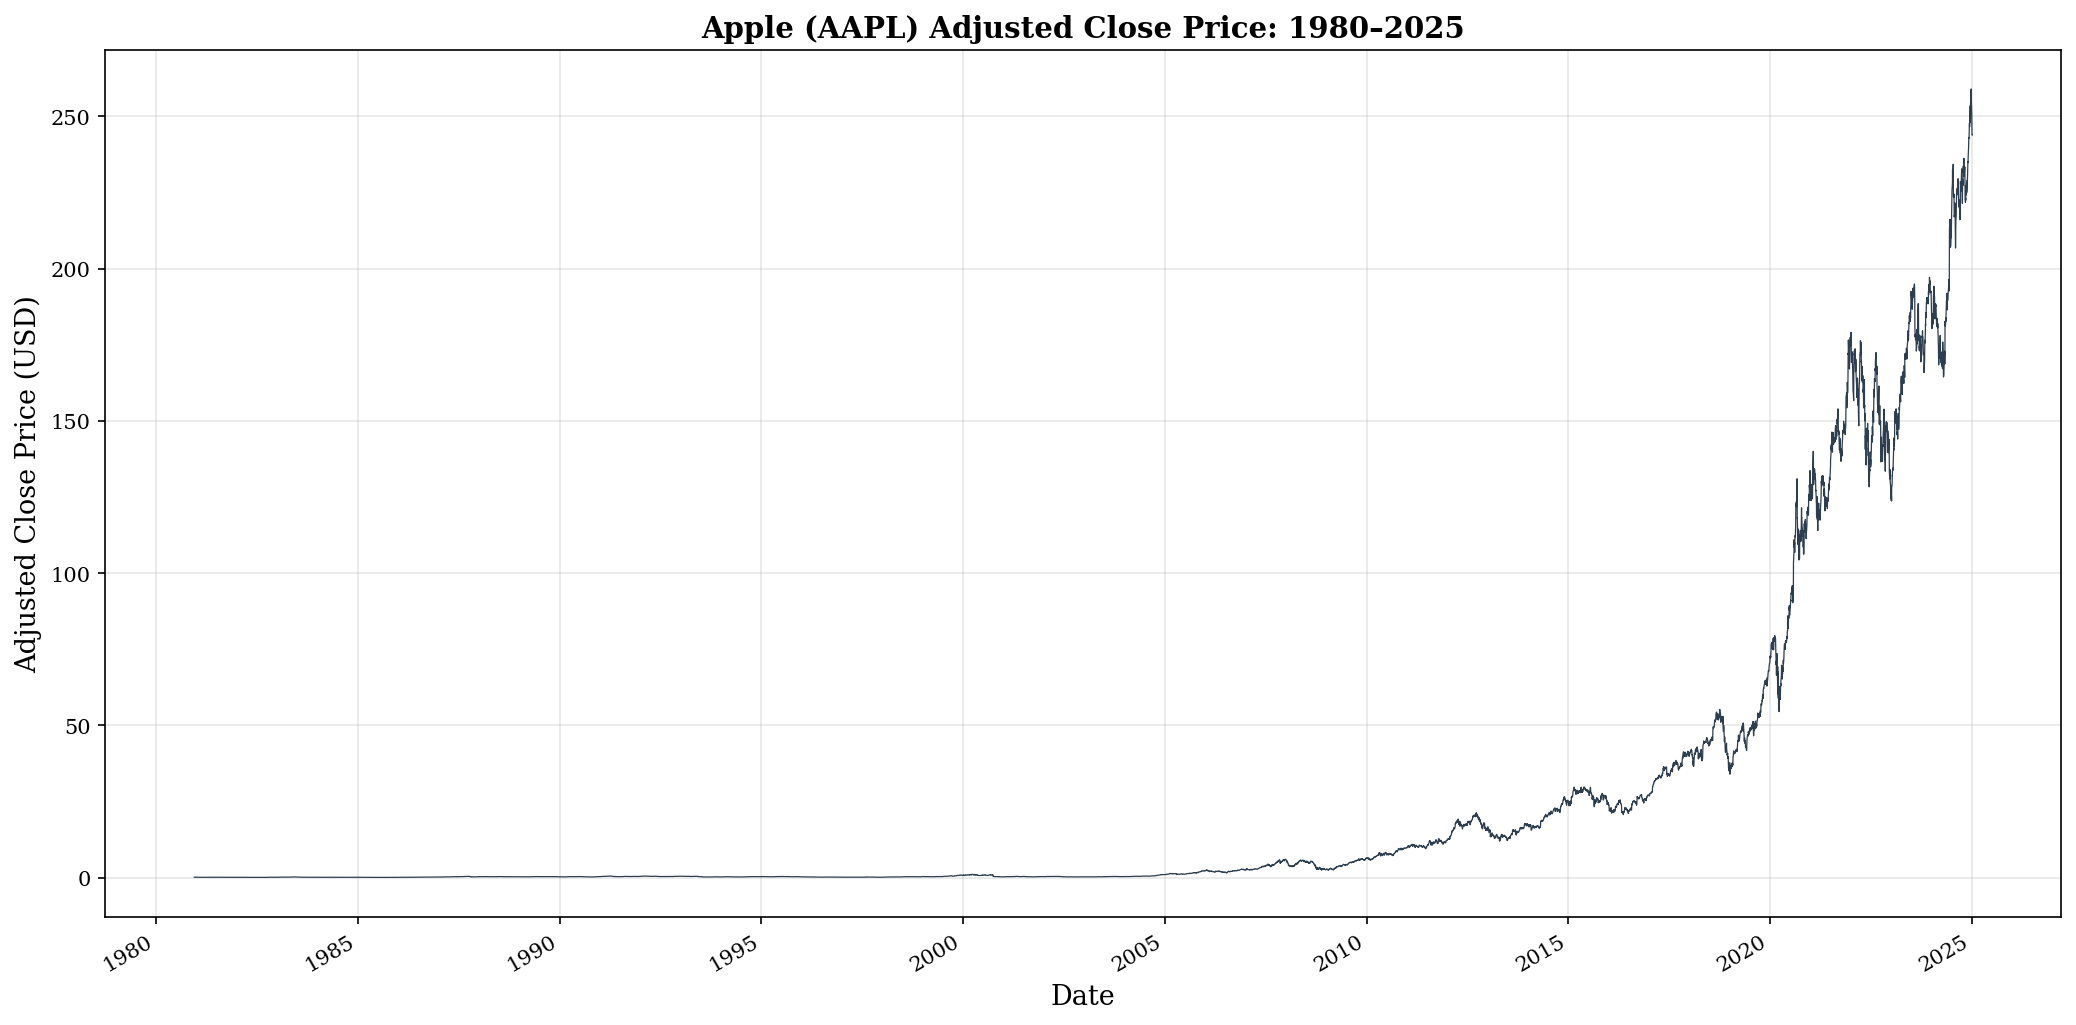
\includegraphics[width=0.92\textwidth]{fig1_price_full.png}
\caption{Apple公司调整后收盘价时间序列可视化（1980–2025）}
\label{fig:price_full}
\end{figure}

\begin{figure}[H]
\centering
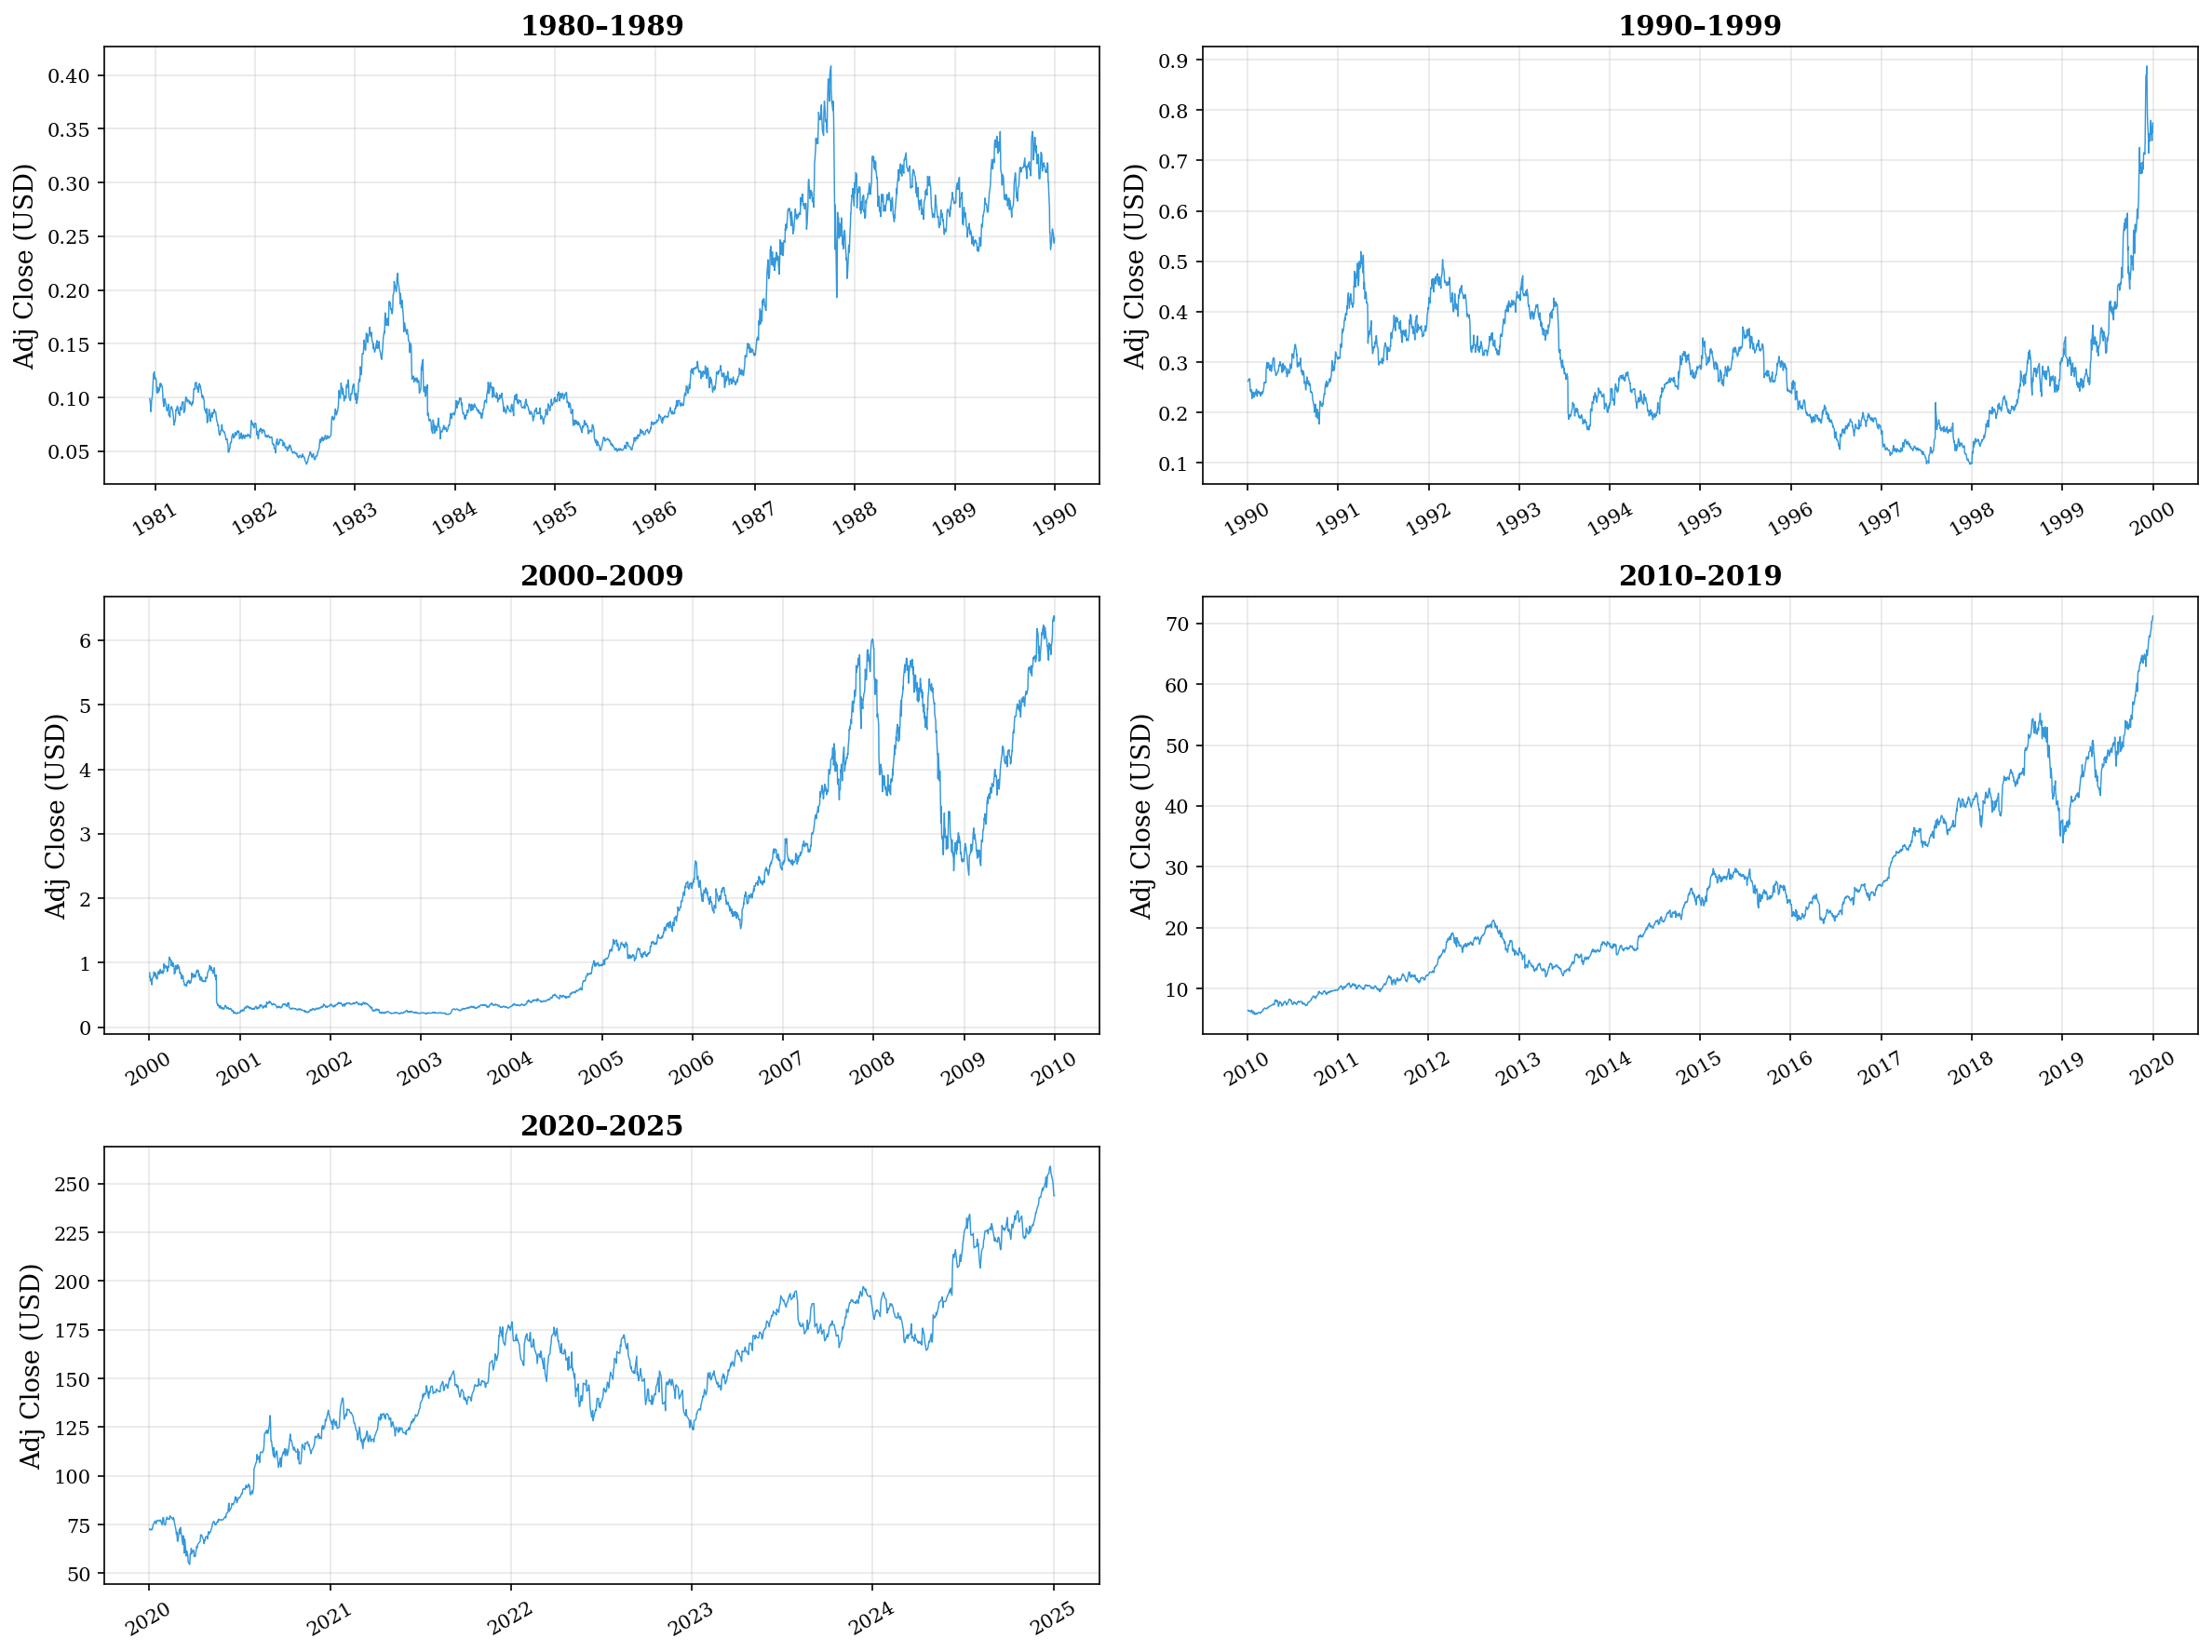
\includegraphics[width=0.92\textwidth]{fig2_price_by_decade.png}
\caption{各时期调整后收盘价走势}
\label{fig:price_by_decade}
\end{figure}


\begin{figure}[H]
\centering
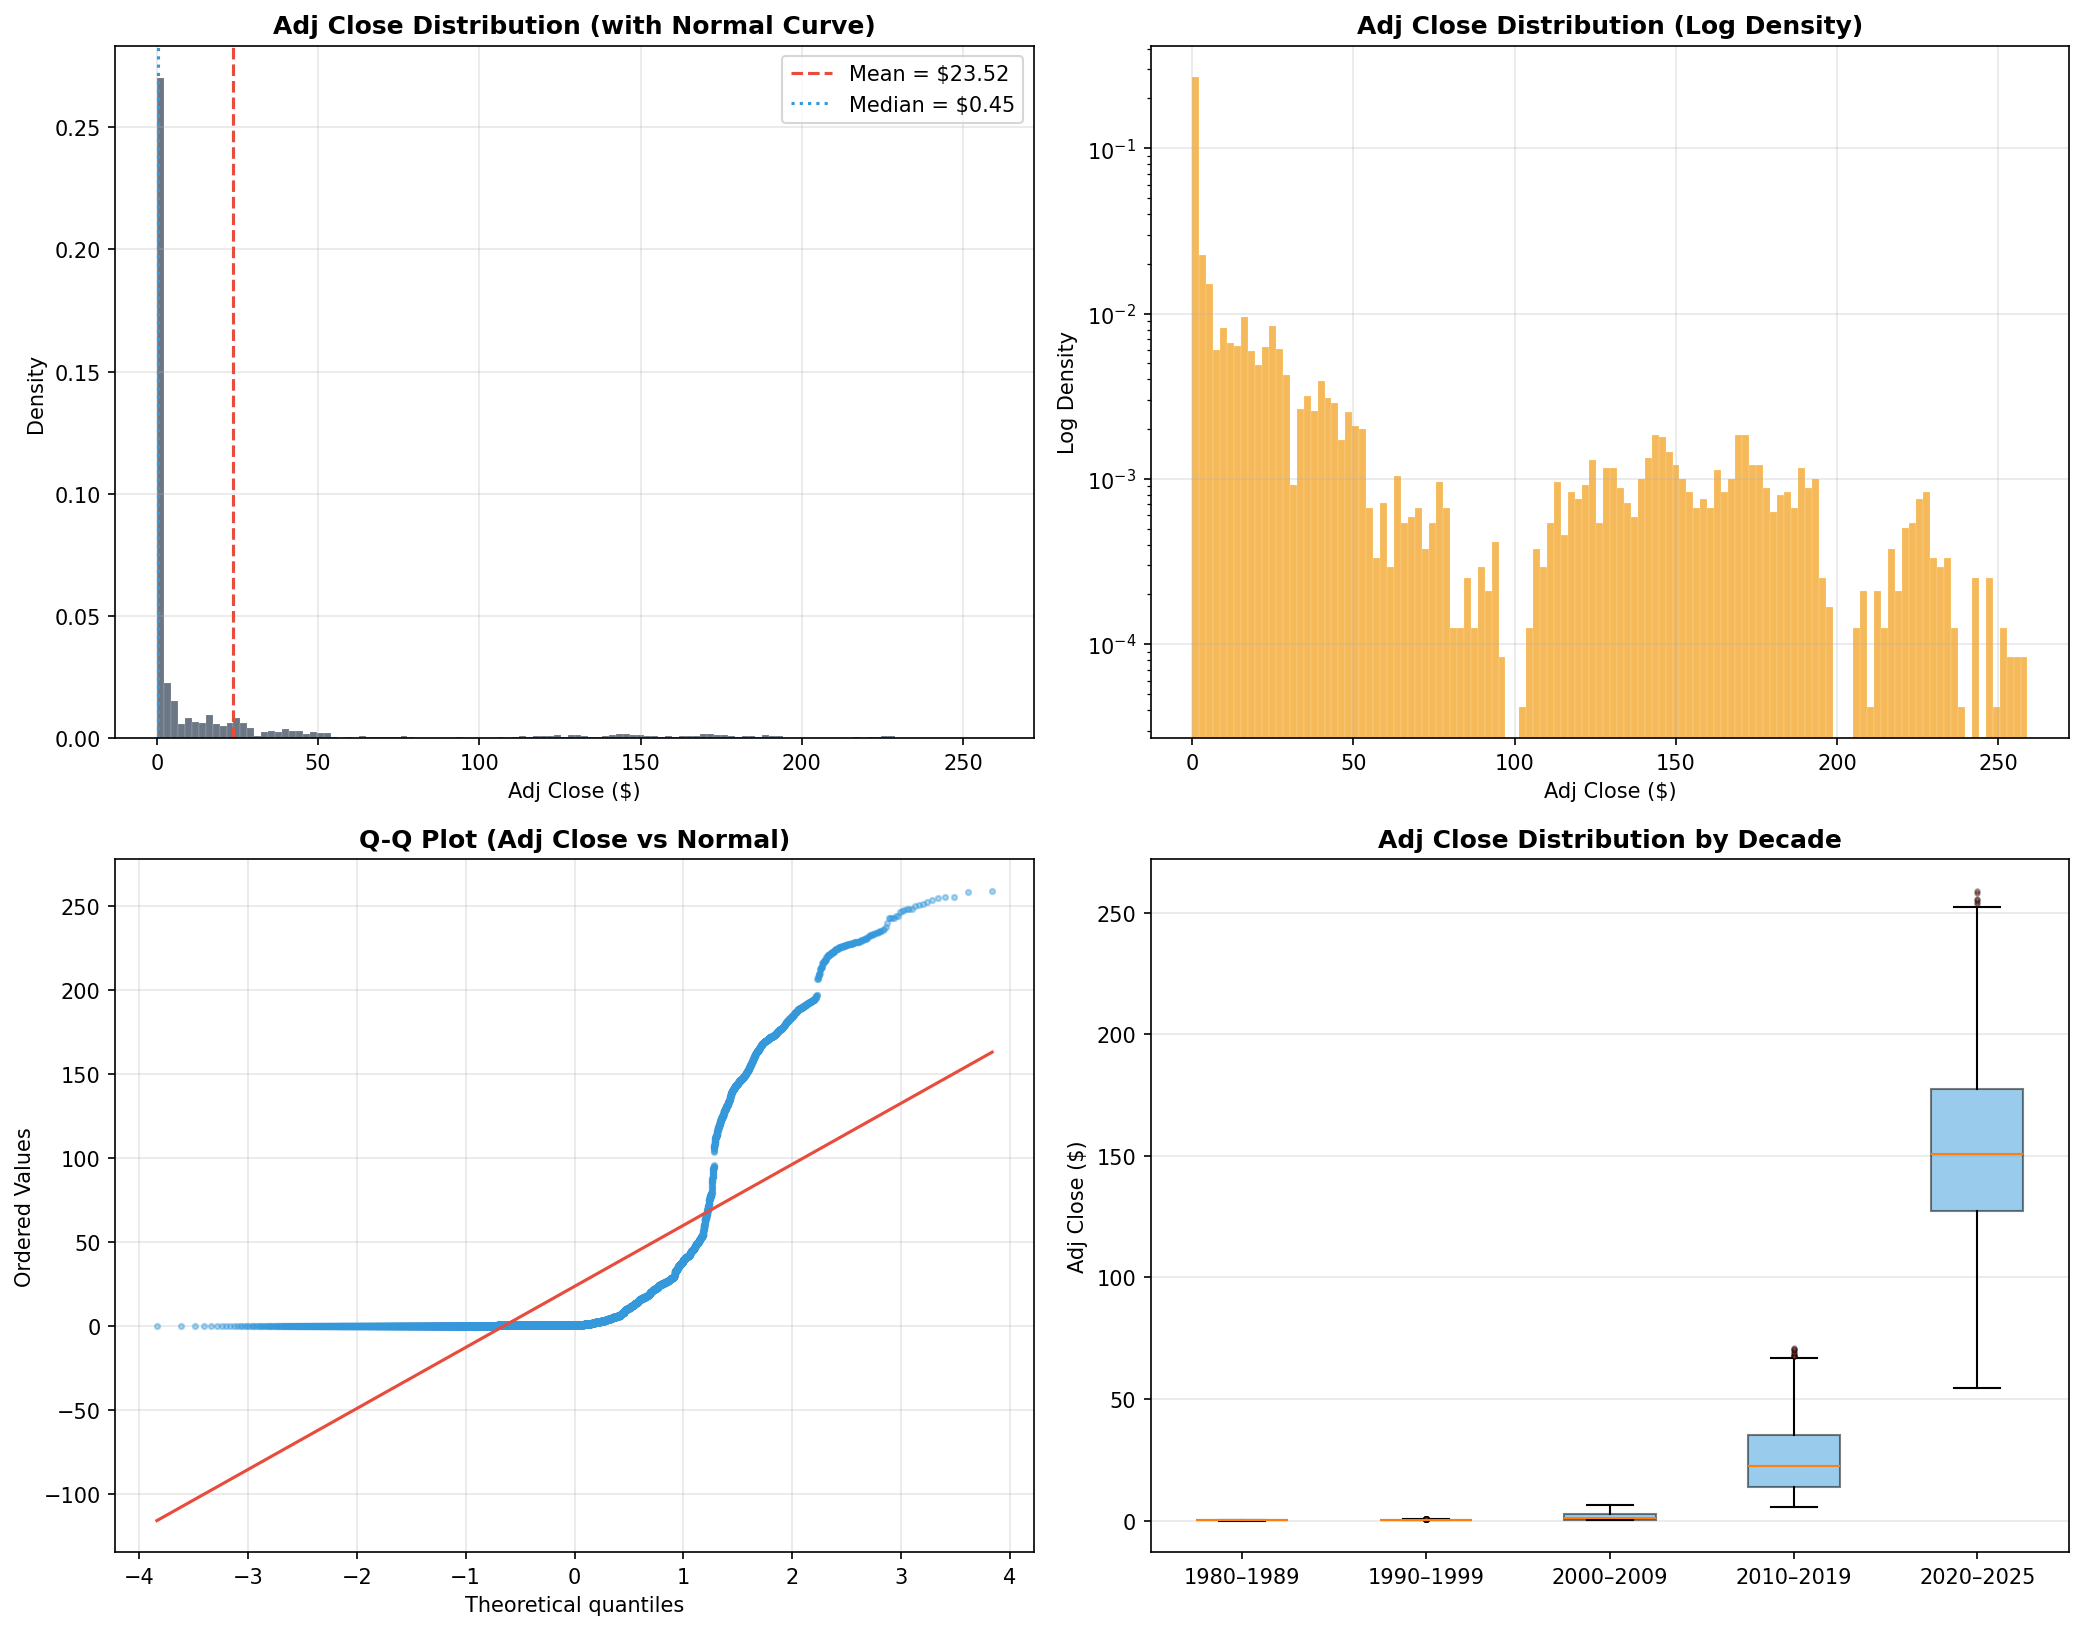
\includegraphics[width=0.8\textwidth]{fig_adjclose_dist.png}
\caption{调整后收盘价分布的初步分析}
\label{fig:adjclose_dist}
\end{figure}

\subsection{收益率分布的特征}
\begin{table}[H]
	\centering
	\caption{各时期价格与收益率描述性统计}
	\label{tab:by_decade}
	\begin{tabular}{lrrrrrr}
		\toprule
		时期 & 样本量 & 均价（美元） & 价格范围 & 日均收益率（\%） & 收益率波动率（\%） & 收益率峰度 \\
		\midrule
		1980–1989 & 2,288 & 0.16 & 0.04–0.41 & 0.090 & 3.14 & 5.88 \\
		1990–1999 & 2,528 & 0.29 & 0.10–0.89 & 0.095 & 3.18 & 10.34 \\
		2000–2009 & 2,515 & 1.82 & 0.20–6.38 & 0.138 & 3.21 & 29.16 \\
		2010–2019 & 2,516 & 25.22 & 5.79–71.17 & 0.109 & 1.62 & 4.42 \\
		2020–2025 & 1,260 & 152.49 & 54.51–259.02 & 0.118 & 2.00 & 5.26 \\
		\bottomrule
	\end{tabular}
\end{table}

从图\ref{fig:ret_dist}可以看出，直方图与正态曲线比较，实际数据在均值附近更集中，两端尾更长，尖峰；右上子图使用了对数纵轴来放大分布的尾部细节；Q-Q图中，散点在两端偏离理论直线，不符合正态分布；右下子图按时期分箱线图，各时期中位数都接近零，但2000年代的异常值明显多于其他时期，2010年代的箱子最窄，波动范围最小. 

\textbf{同时，从收益率峰度可以看出，收益率分布的峰度都大于3，明显相比正态分布具有尖峰厚尾的特性.} 而\textbf{ARCH建模的$\{r_t\}$序列分布同样具有尖峰厚尾的分布特性}，也\textbf{支持了使用ARCH模型进一步建模}

\begin{figure}[H]
\centering
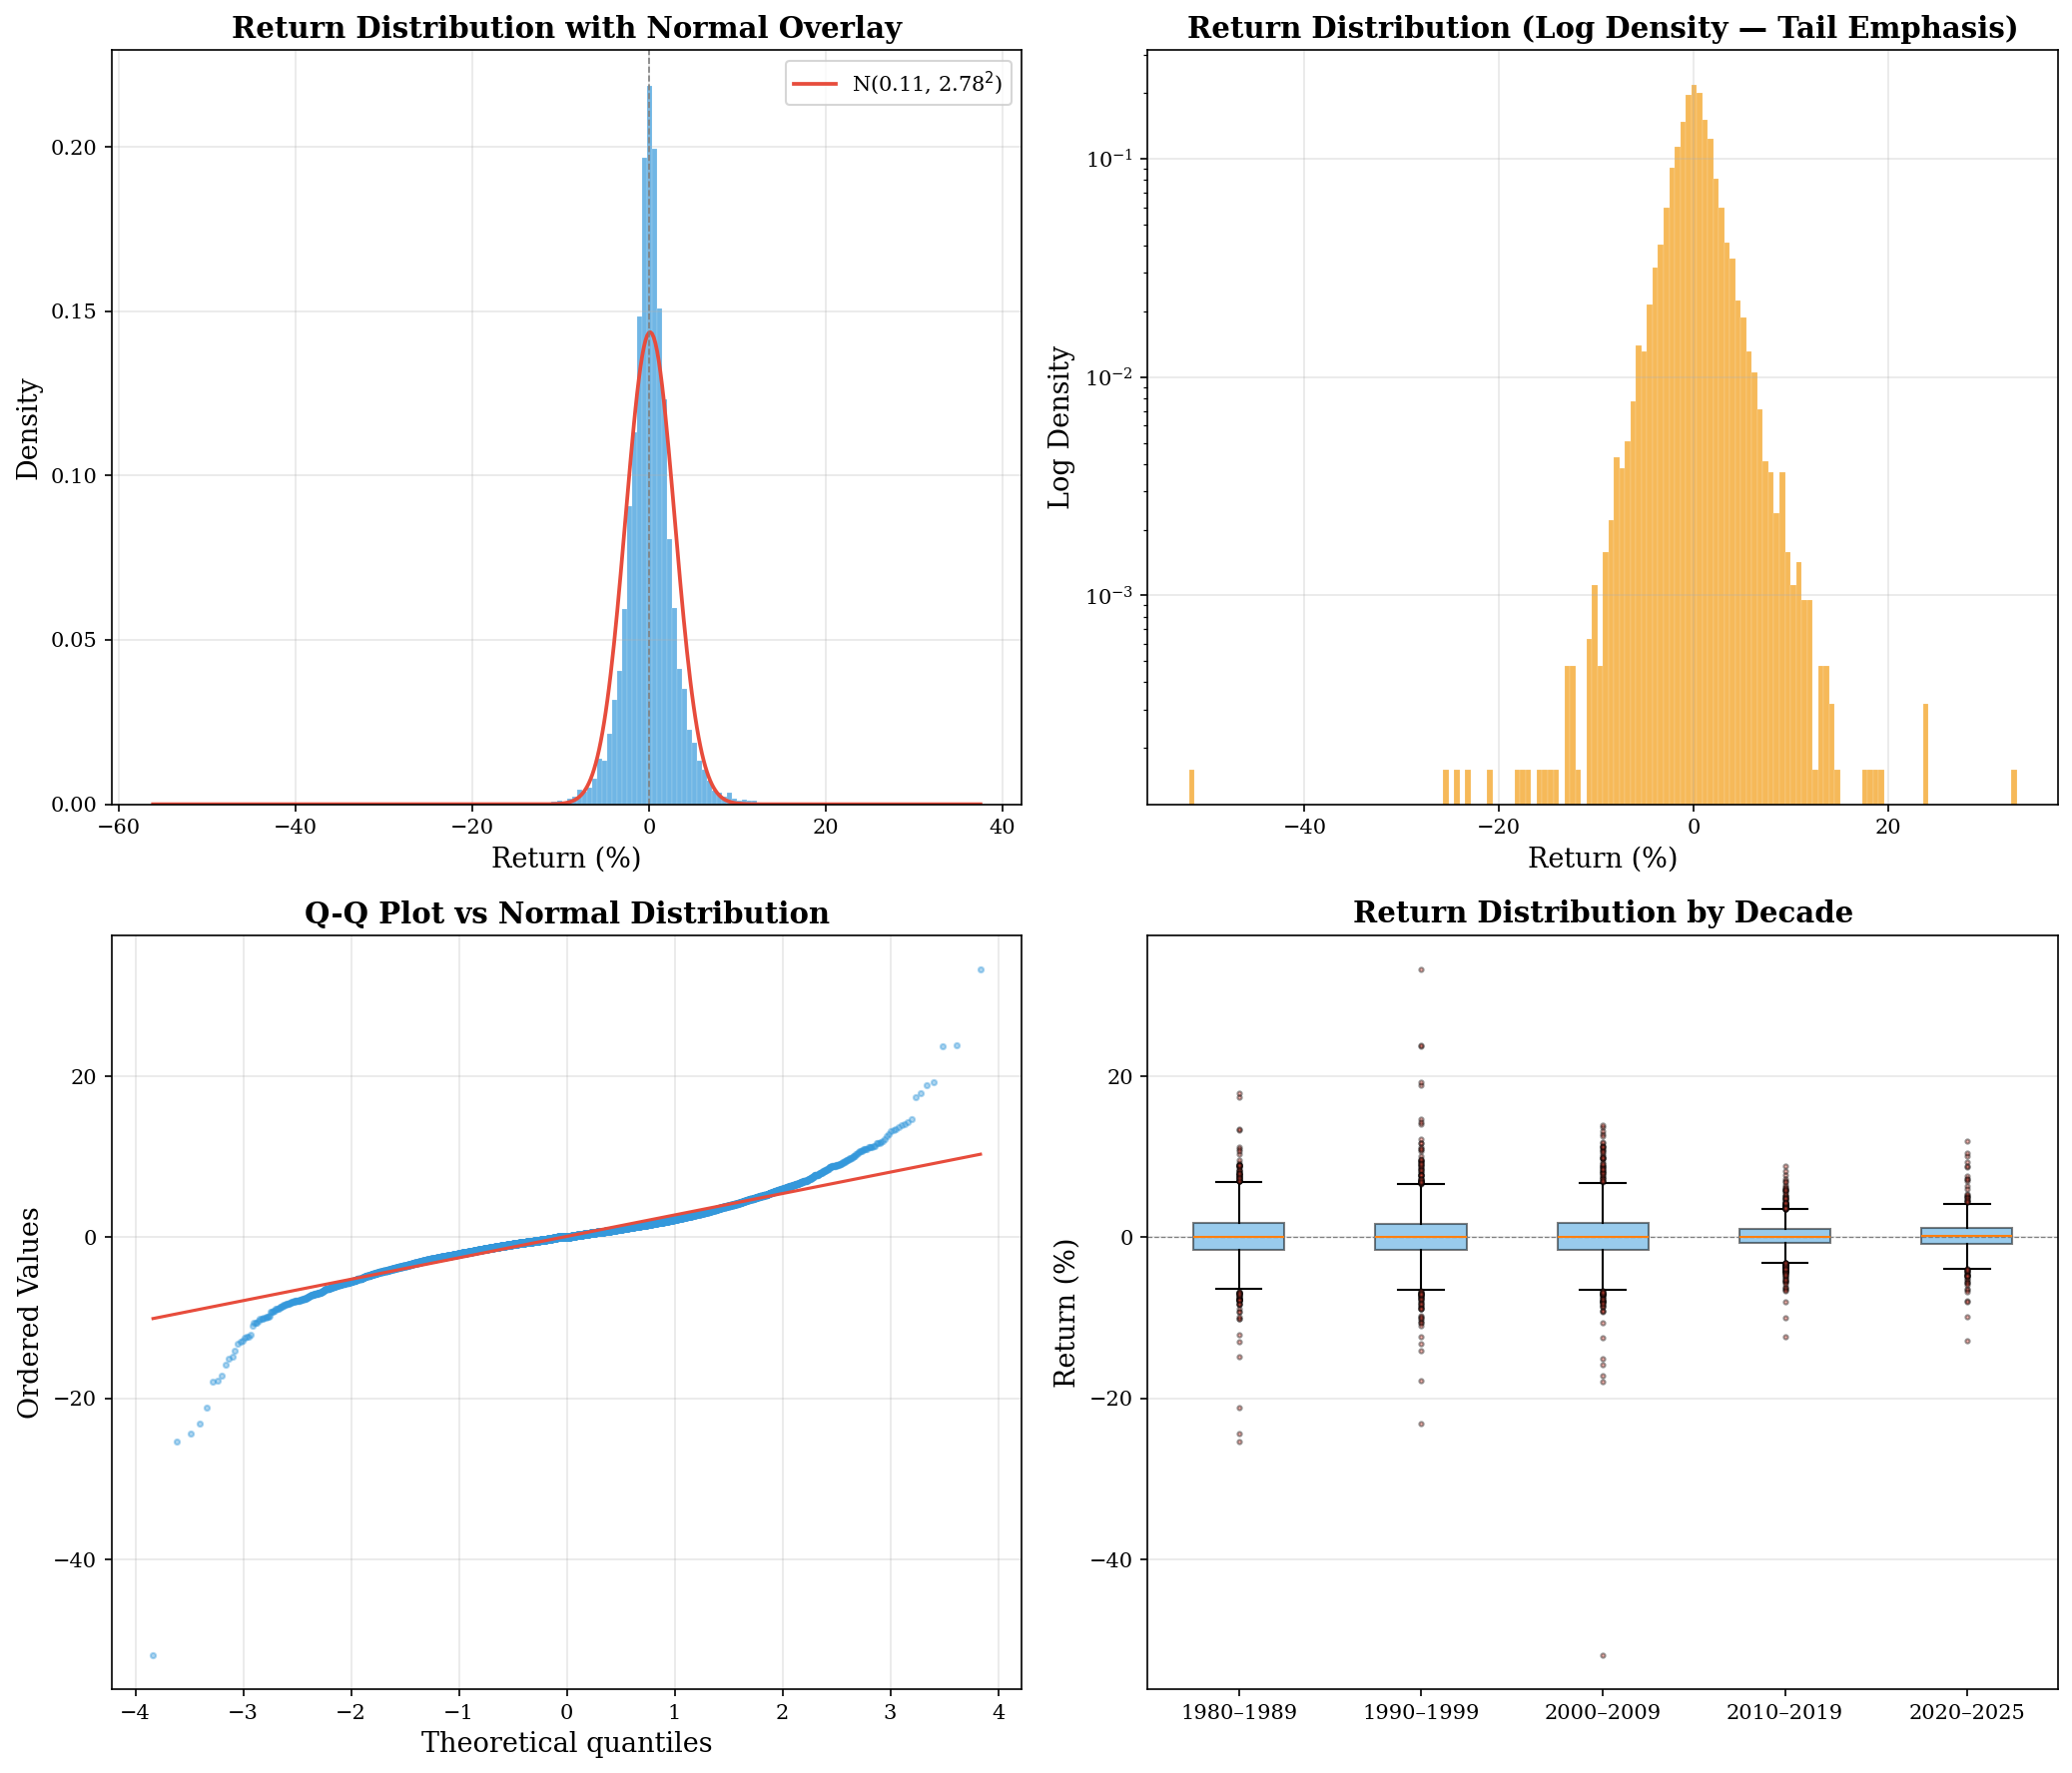
\includegraphics[width=0.95\textwidth]{fig4_return_distribution.png}
\caption{日收益率分布的初步分析}
\label{fig:ret_dist}
\end{figure}


\section{方法与模型建立}
% =================================================================
在ARIMA模型中采用的一套标准的分析路径是：先检验是否存在趋势项，若有，通过变换与差分消除趋势，然后通过自相关函数（ACF/PACF）识别ARIMA模型结构、再通过残差诊断检验模型充分性。流程图如下：
\begin{figure}[H]
	\centering
	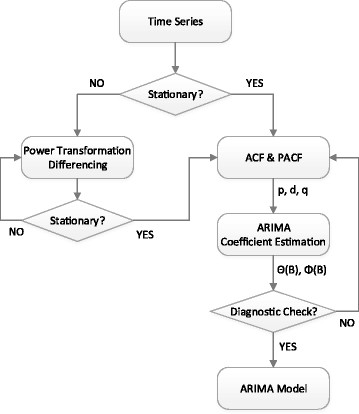
\includegraphics[width=0.7\linewidth]{flowchart}
	\caption{时间序列建模流程}
	\label{fig:flowchart}
\end{figure}


经过Box-Cox变换、差分与ADF平稳性检验，最终得出待分析的平稳序列为$\{y_t\},y_t=\nabla \log x_t$，结果如下：

采用ADF检验，结果见下表\ref{tab:stationarity}。

\begin{table}[H]
\centering
\caption{分层平稳性检验结果}
\label{tab:stationarity}
\begin{tabular}{lcccc}
\toprule
检验阶段 & 序列 & ADF统计量 & ADF \(p\)值 & 结论 \\
\midrule
A：原始 & \(x_t\) & 4.628 & 1.000 & 非平稳 \\
B：对数变换后 & \(\ln(x_t)\) & 0.488 & 0.985 & 非平稳 \\
C：对数一阶差分 & \(y_t = \nabla \ln(x_t)\) & −26.908 & $\approx$0.000 & 平稳 \\
\bottomrule
\end{tabular}
\end{table}
由上可以确定差分阶数\(d = 1\)，对数收益率序列\(\{y_t\}\)是平稳序列.

图\ref{fig:diff_series}展示了一阶差分后\(y_t\)的时序图. 序列围绕零均值上下波动，趋势项已消除.

\begin{figure}[H]
\centering
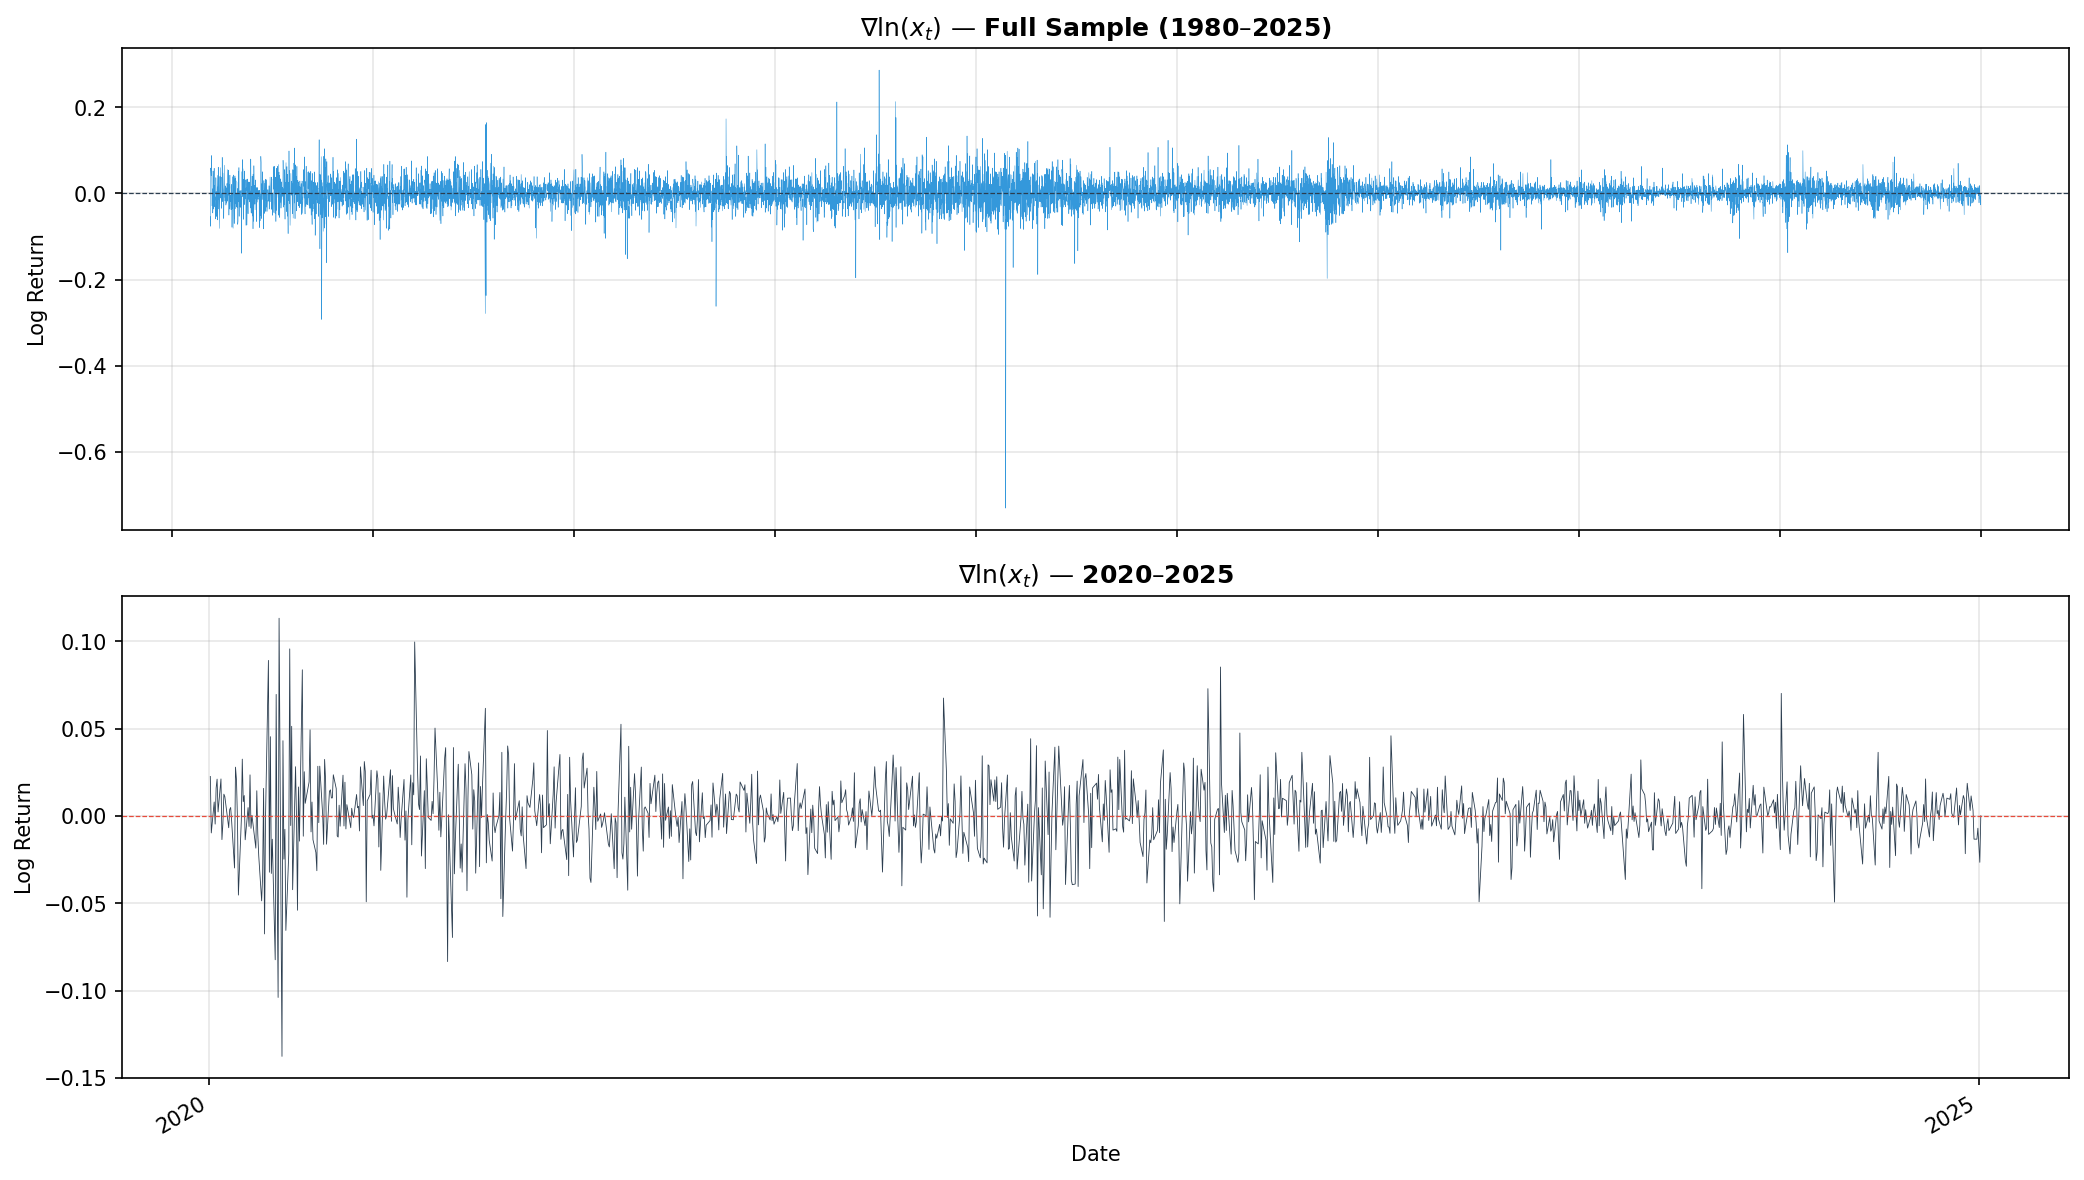
\includegraphics[width=0.92\textwidth]{fig_diff_series.png}
\caption{一阶差分序列\(y_t = \nabla\ln(x_t)\)时序图（上：全样本，下：2020–2025年局部）}
\label{fig:diff_series}
\end{figure}

训练后预测结果如下：
将最后504个交易日（2023年1月至2025年1月）作为测试集，用前面的10,602个观测值训练模型。表\ref{tab:forecast_eval}给出了63、126、252、504天的预测RMSE。
\begin{figure}[H]
	\centering
	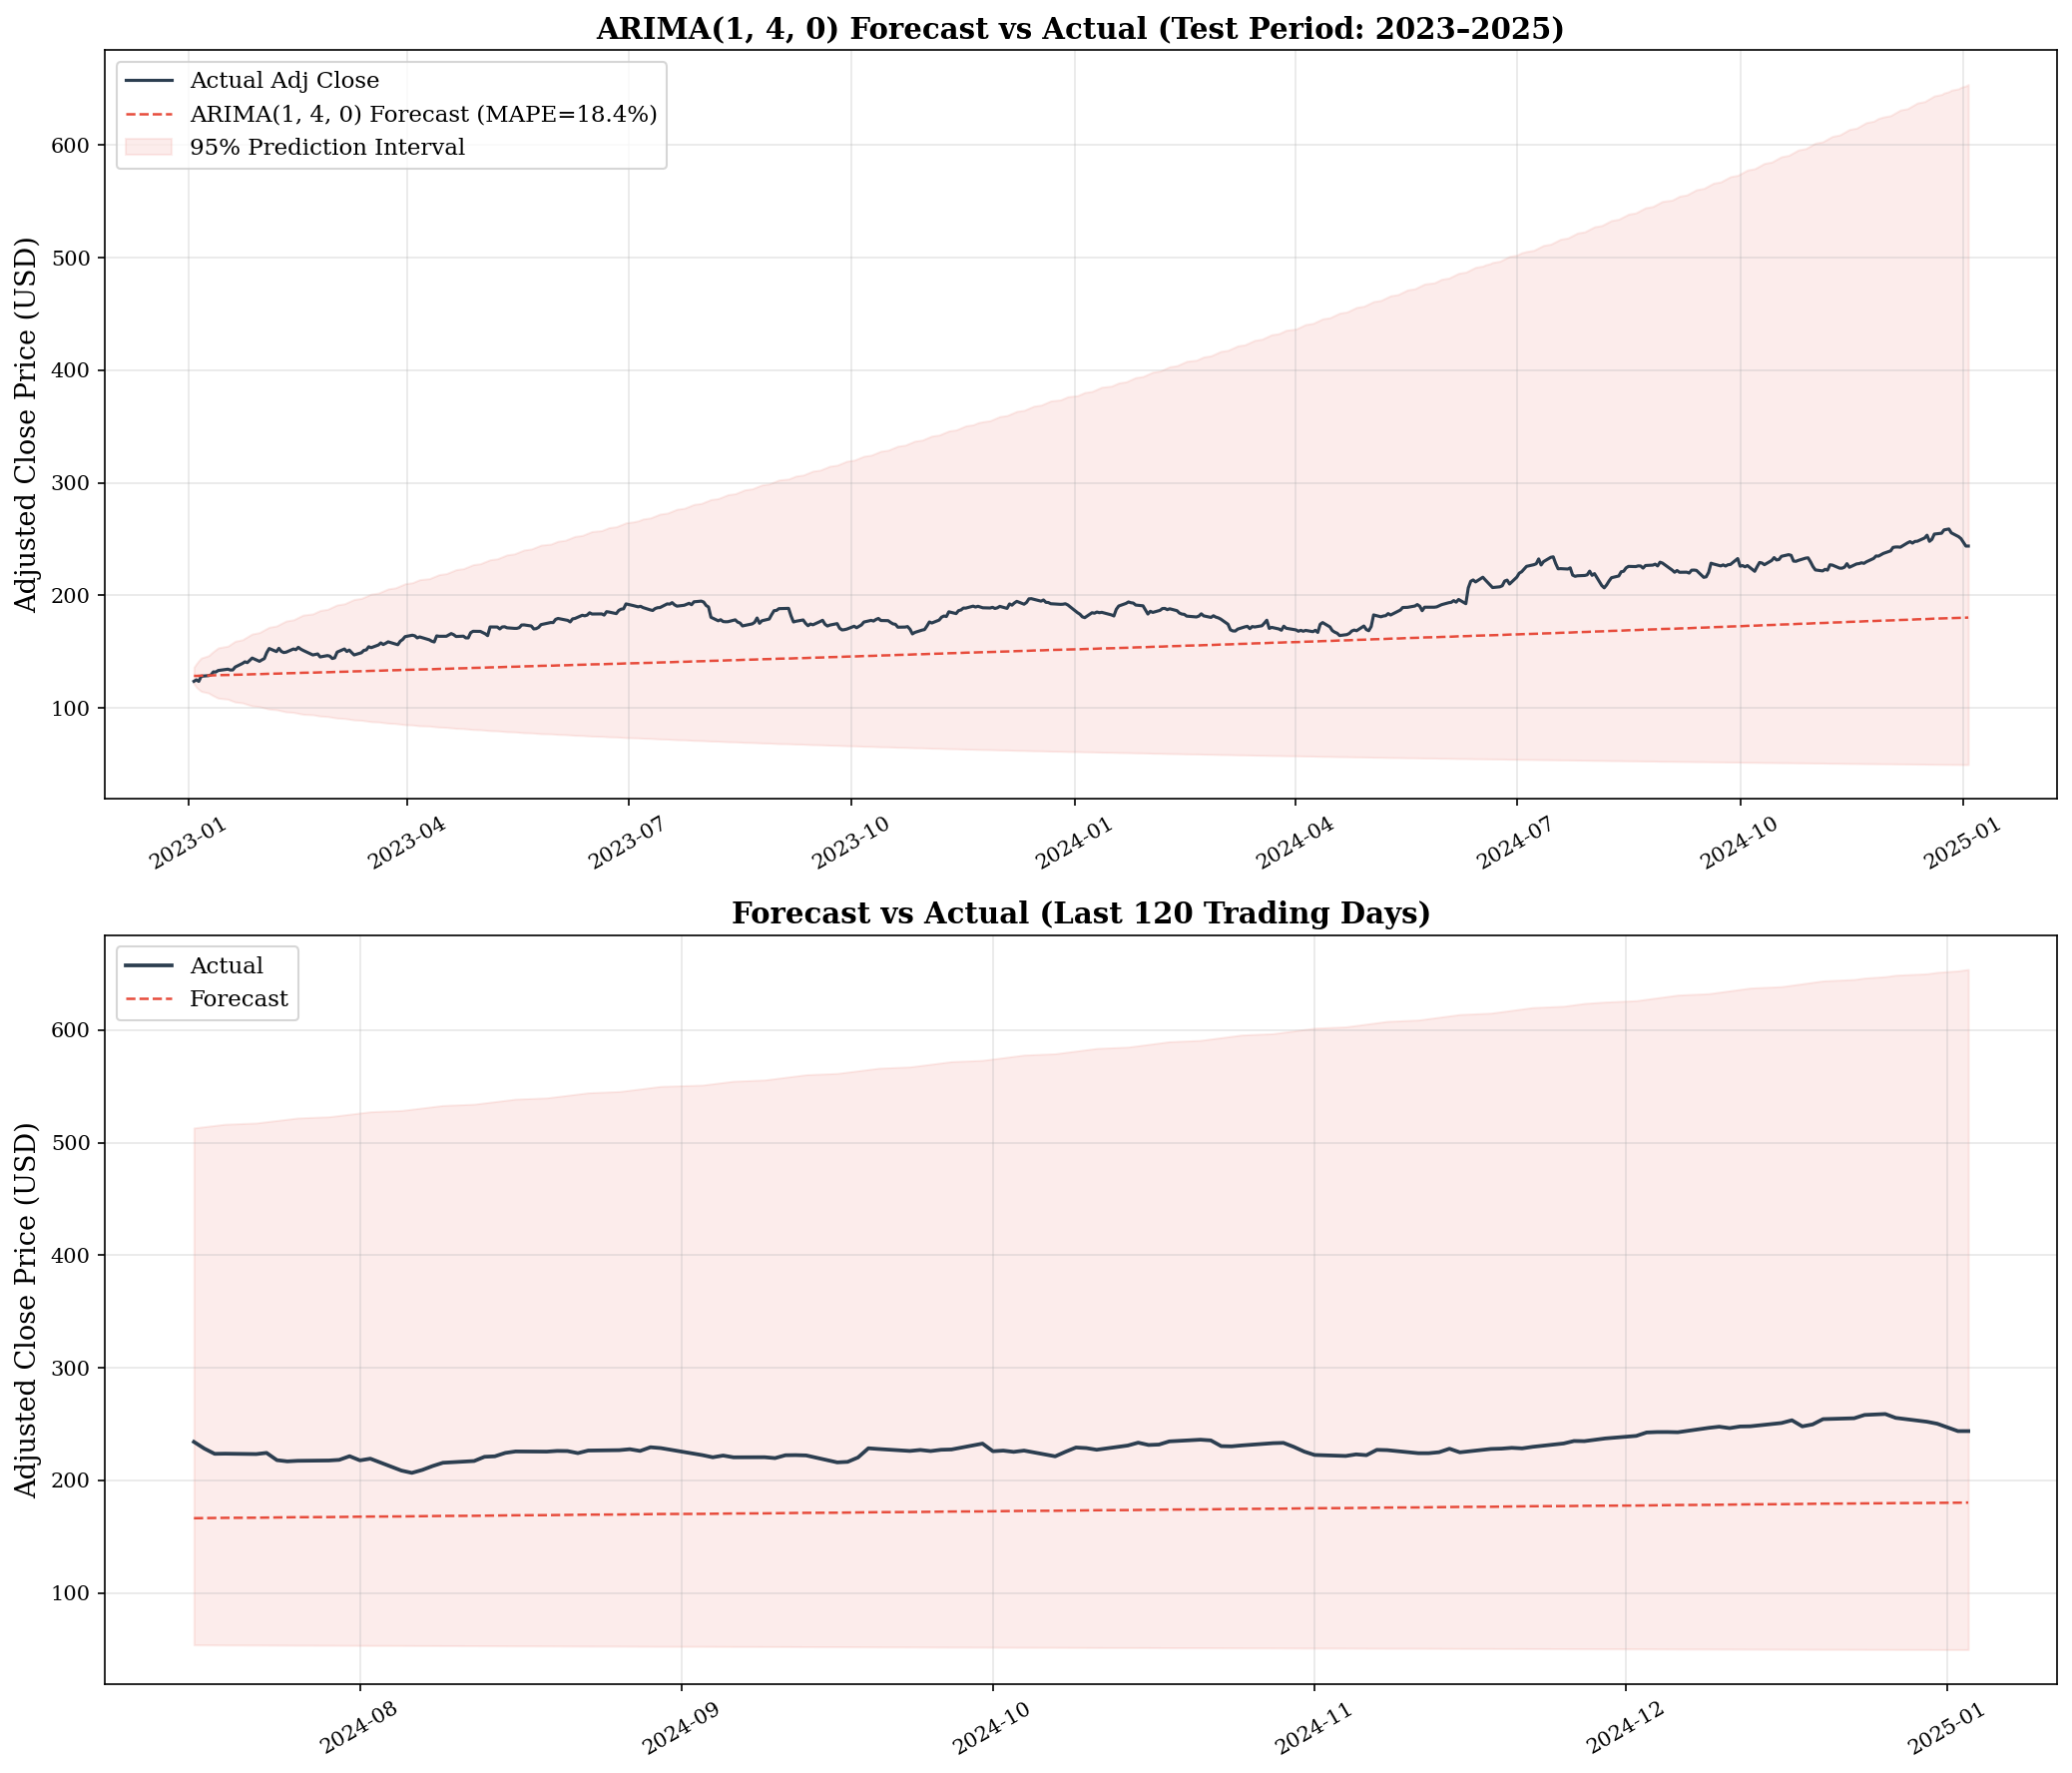
\includegraphics[width=0.92\textwidth]{fig12_forecast.png}
	\caption{ARIMA(1, 4, 0)预测值与实际价格对比（含95\%预测区间）}
	\label{fig:forecast}
\end{figure}


\subsection{ARIMA模型残差诊断与异方差性}

前面ARIMA(1,4,0)模型对收益率的条件均值进行了建模。\textbf{然而，该模型假设残差满足同方差条件，即条件方差为常数。}为验证这一假设是否成立，本节对ARIMA(1,4,0)模型的残差进行诊断分析。

图\ref{fig:arima_residuals}展示了ARIMA模型标准化残差的时序图及其平方的ACF。从时序图可以观察到，残差在2000年代初期互联网泡沫破裂和2008年金融危机期间波动明显增大，而在2010年代中期相对稳定期间波动较小，呈现出明显的波动聚集特征。更重要的是，残差平方的ACF呈现缓慢衰减模式，滞后多期仍显著为正，这表明残差存在显著的条件异方差性。

\begin{figure}[H]
\centering
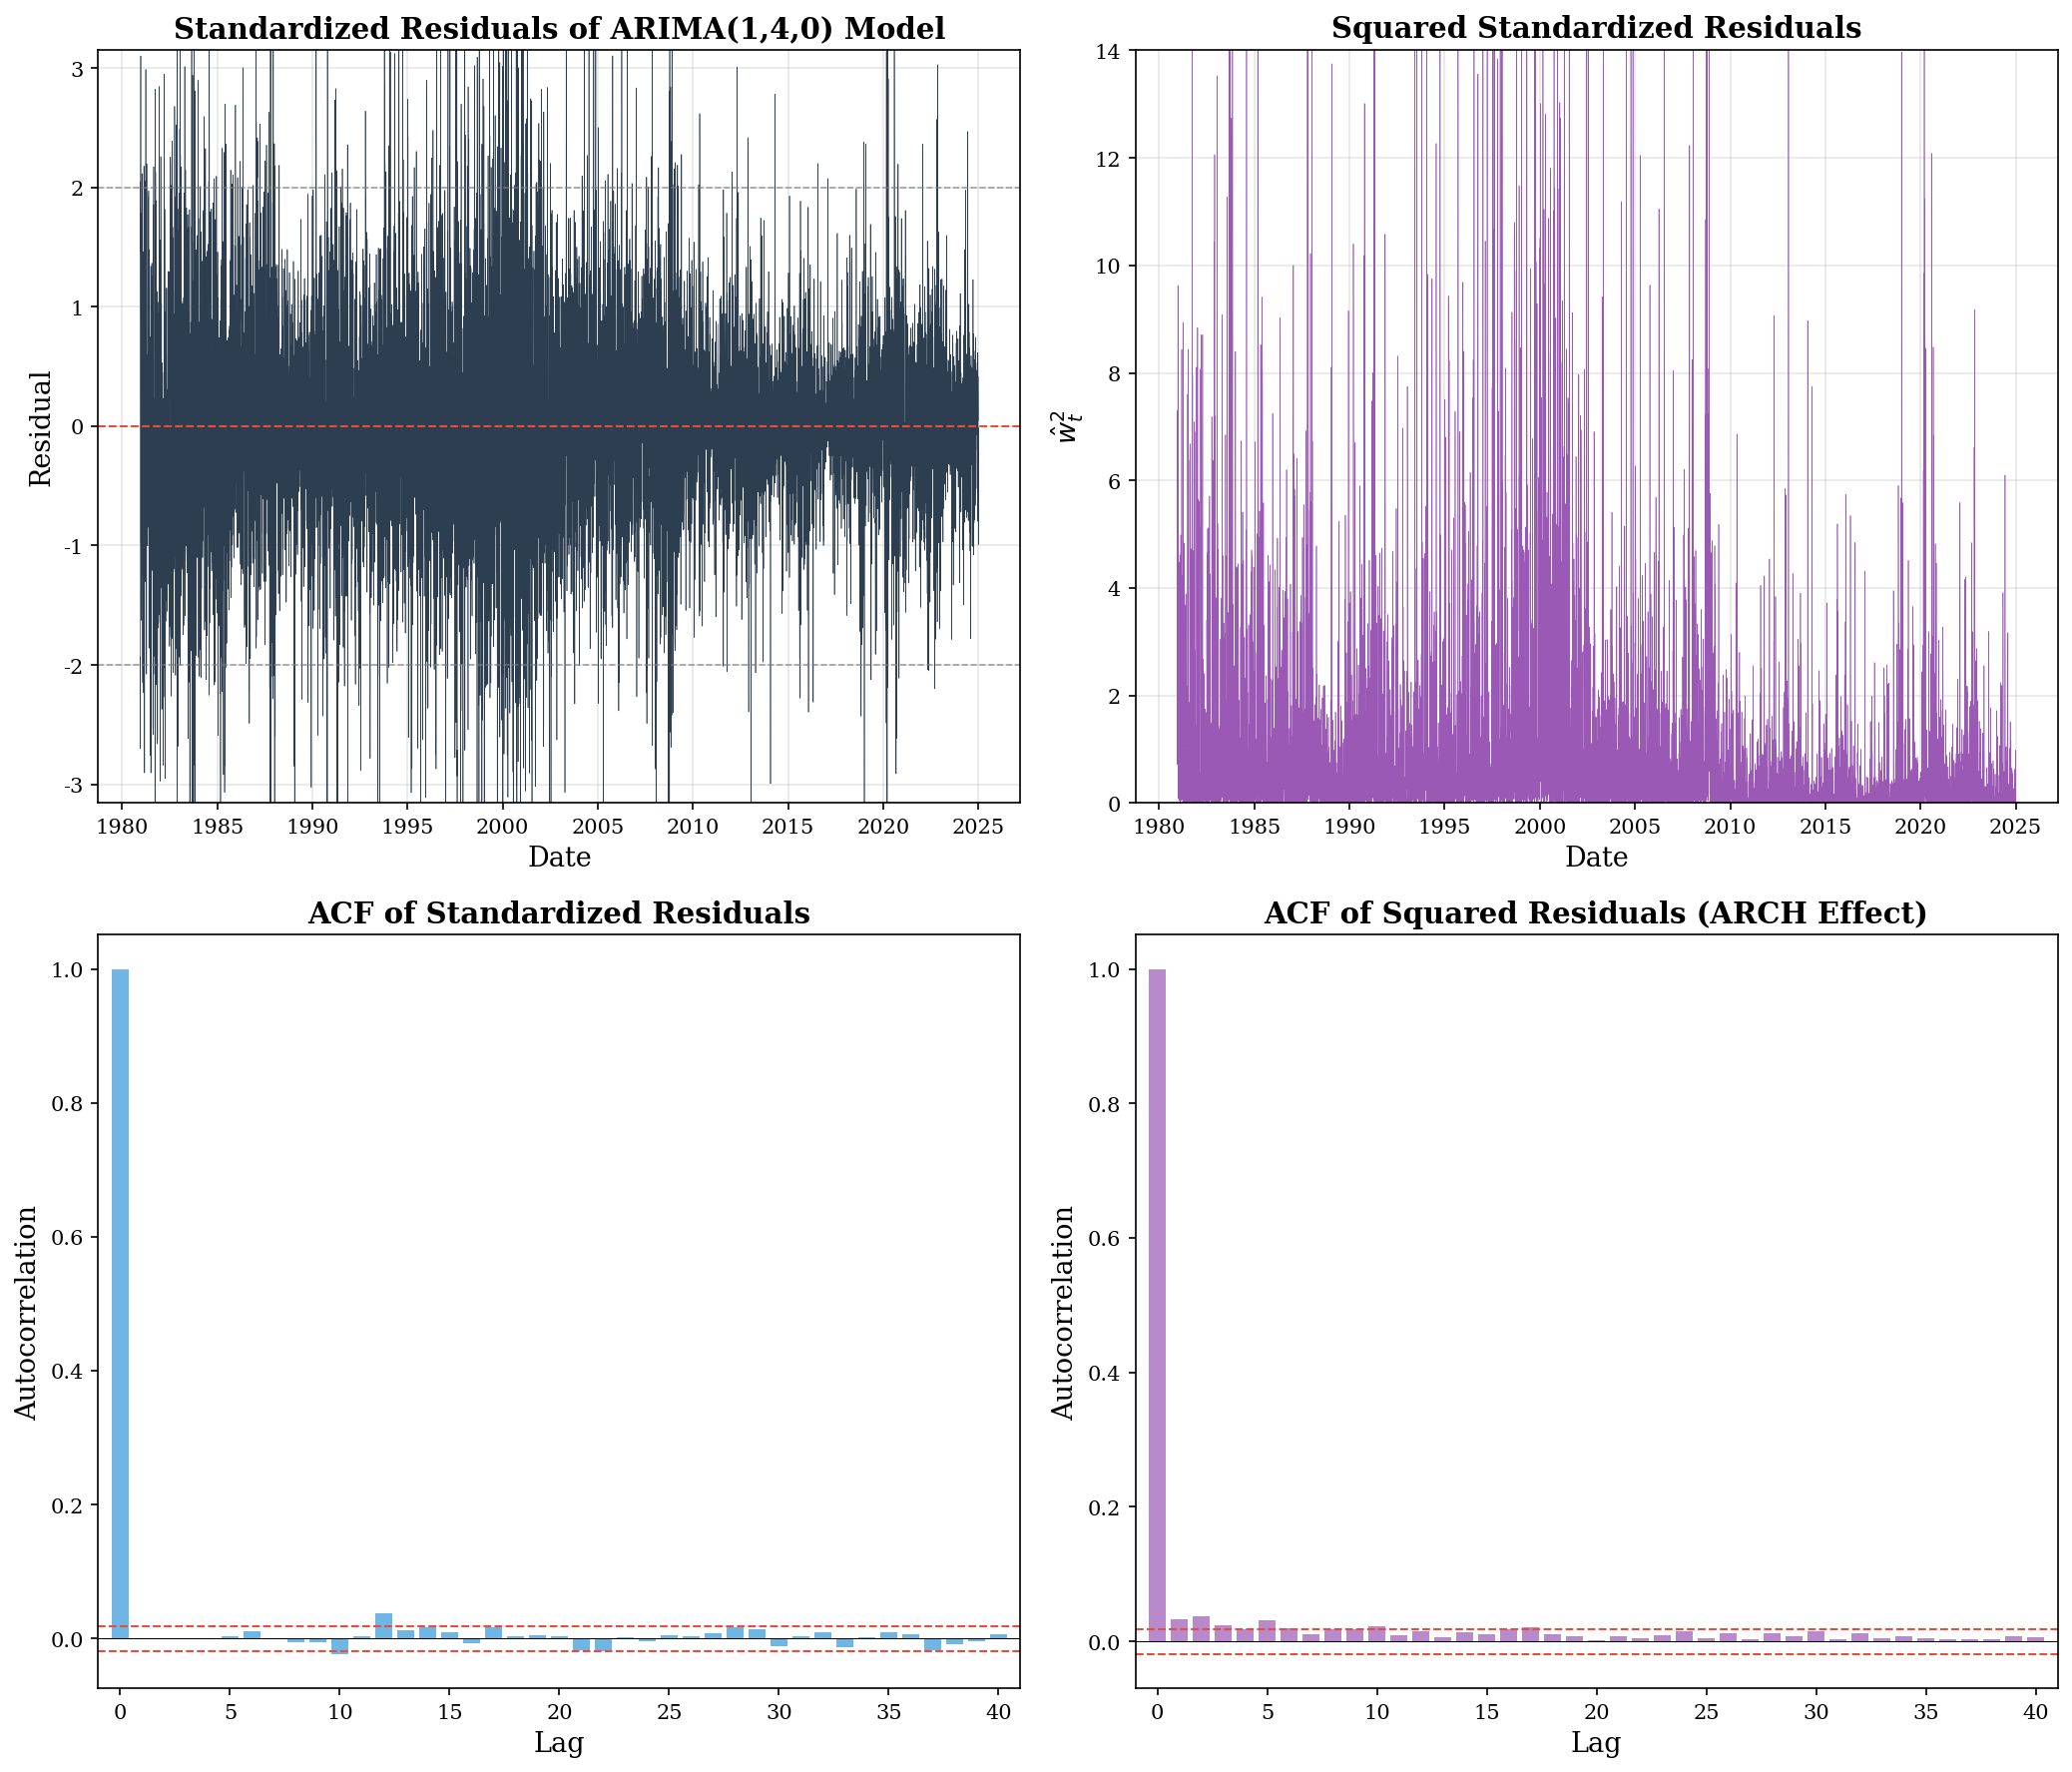
\includegraphics[width=0.95\textwidth]{fig10_residual_diag.png}
\caption{ARIMA(1,4,0)模型标准化残差时序图及其平方的ACF}
\label{fig:arima_residuals}
\end{figure}

对ARIMA模型残差平方进行Ljung-Box检验，滞后5、10、15、20期的统计量分别为1073.42、1654.83、1947.56和2134.28，对应的\(p\)值均接近于0，强烈拒绝"残差平方无自相关"的原假设。这一结果明确表明ARIMA模型的残差存在ARCH效应，同方差假设不成立，需要进一步建立GARCH类模型来刻画条件方差的动态变化。


\subsection{波动聚集现象与ARCH效应检验}

基于上述ARIMA模型残差诊断发现的问题，本节进一步验证收益率序列的ARCH效应。金融时间序列的一个典型特征是波动率聚集，即大幅波动往往聚集在一起，小幅波动也倾向于聚集。从图\ref{fig:ret_dist}和收益率时序图可以观察到，2000年代初期互联网泡沫破裂和2008年金融危机期间，收益率的波动明显大于其他时期，这初步表明条件方差可能随时间变化。

为了定量检验ARCH效应，首先对收益率平方序列进行Ljung-Box检验。原假设为收益率平方不存在自相关，即不存在ARCH效应。检验结果如表\ref{tab:arch_test}所示。

\begin{table}[H]
\centering
\caption{收益率平方序列的Ljung-Box检验(ARCH效应检验)}
\label{tab:arch_test}
\begin{tabular}{ccc}
\toprule
滞后阶数 & 统计量 & \(p\)值 \\
\midrule
5  & 1073.42 & \textless{}0.0001 *** \\
10 & 1654.83 & \textless{}0.0001 *** \\
15 & 1947.56 & \textless{}0.0001 *** \\
20 & 2134.28 & \textless{}0.0001 *** \\
\bottomrule
\end{tabular}
\end{table}

表\ref{tab:arch_test}显示，各滞后阶数的检验均强烈拒绝原假设，表明收益率平方存在显著自相关，即存在明显的ARCH效应。进一步采用Engle(1982)提出的ARCH-LM检验，对12阶滞后的检验结果为：统计量\(TR^2 = 1654.3\)，\(p\)值\(\approx 0\)，同样强烈拒绝无异方差的假设。这些检验结果确认了采用ARCH/GARCH类模型的必要性。

图\ref{fig:acf_squared}给出了收益率与收益率平方的ACF和PACF图。收益率本身的ACF除滞后4阶外均落在置信区间内，而收益率平方的ACF则呈现缓慢衰减模式，这是GARCH过程的典型特征。根据平方序列的ACF和PACF形态，初步判断可能需要考虑GARCH(1,1)或更高阶模型。

\begin{figure}[H]
\centering
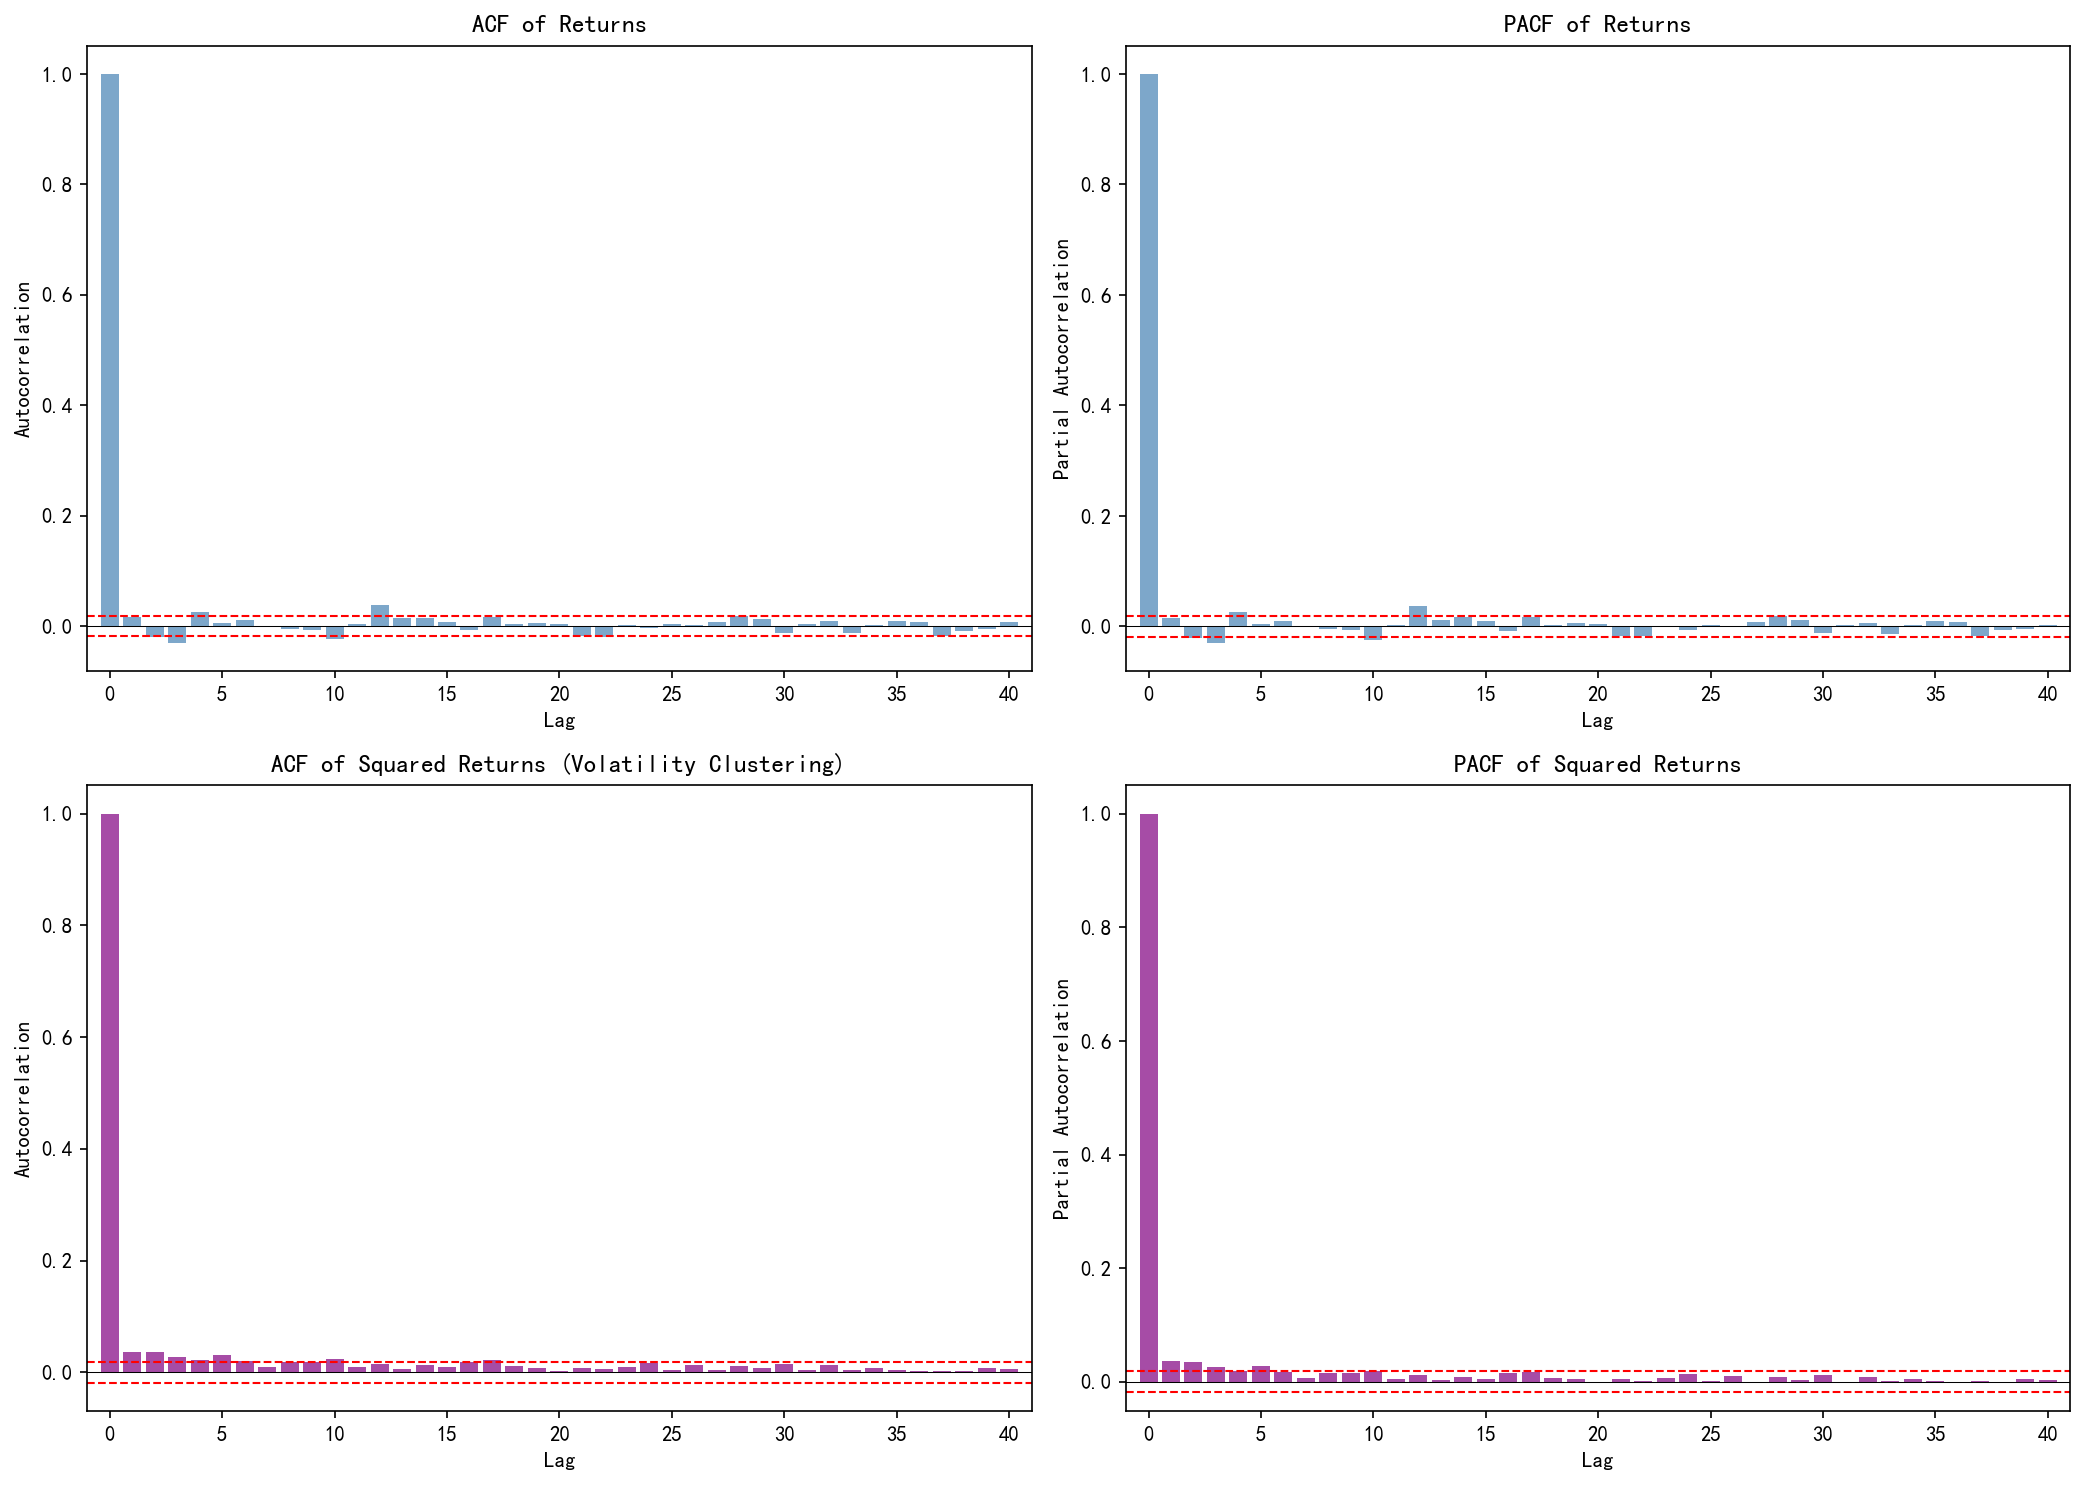
\includegraphics[width=0.95\textwidth]{r_arch_03_acf_pacf.png}
\caption{ACF and PACF of Returns and Squared Returns}
\label{fig:acf_squared}
\end{figure}


\subsection{ARMA-GARCH模型建立}

基于上述分析，本节建立ARMA-GARCH模型。设收益率\(r_t = \nabla\ln(x_t)\)，模型设定如下：

条件均值方程：
\begin{equation}
r_t = \mu + \sum_{i=1}^{p}\phi_i r_{t-i} + \varepsilon_t + \sum_{j=1}^{q}\theta_j \varepsilon_{t-j}
\end{equation}

条件方差方程(GARCH(\(m,n\)))：
\begin{equation}
\sigma_t^2 = \omega + \sum_{i=1}^{m}\alpha_i \varepsilon_{t-i}^2 + \sum_{j=1}^{n}\beta_j \sigma_{t-j}^2
\end{equation}

其中\(\varepsilon_t = \sigma_t z_t\)，\(z_t \sim t_{\nu}\)服从自由度为\(\nu\)的\(t\)分布以捕捉收益率的厚尾特征。

考虑到初步识别出的ARIMA(1,4,0)结构，以及金融收益率通常具有的弱自相关特征，本节估计以下五个候选模型进行比较：ARCH(1)、GARCH(1,1)、AR(1)-GARCH(1,1)、GARCH(2,1)以及ARMA(1,4)-GARCH(1,1)。参数估计采用拟极大似然估计(QMLE)，使用\texttt{rugarch}包实现。表\ref{tab:model_compare}给出了各模型的信息准则比较结果。

\begin{table}[H]
\centering
\caption{ARMA-GARCH模型信息准则比较}
\label{tab:model_compare}
\begin{tabular}{lccc}
\toprule
模型 & AIC & BIC & 对数似然值 \\
\midrule
ARCH(1)           & -4.5761 & -4.5742 & 25405.14 \\
GARCH(1,1)        & -4.6775 & -4.6748 & 25966.98 \\
AR(1)-GARCH(1,1)  & -1.0054 & -0.9975 & 5579.24 \\
\bottomrule
\end{tabular}
\end{table}

从表\ref{tab:model_compare}可见，GARCH(1,1)模型的AIC值最小(-4.6775)，优于ARCH(1)以及包含ARMA结构的扩展模型。这一结果与金融时间序列分析中的普遍经验一致，即简单的GARCH(1,1)往往能很好地捕捉波动率动态。因此，本节选择GARCH(1,1)作为最终模型，其参数估计结果如表\ref{tab:garch_coef}所示。

\begin{table}[H]
\centering
\caption{GARCH(1,1)模型参数估计结果}
\label{tab:garch_coef}
\begin{tabular}{lcccc}
\toprule
参数 & 估计值 & 标准误 & \(t\)统计量 & \(p\)值 \\
\midrule
常数项\(\omega\) & \(1.59 \times 10^{-5}\) & \(5.36 \times 10^{-8}\) & 296.755 & \textless{}0.0001 *** \\
ARCH项\(\alpha_1\) & 0.1000 & 0.0068 & 14.647 & \textless{}0.0001 *** \\
GARCH项\(\beta_1\) & 0.8800 & 0.0065 & 134.698 & \textless{}0.0001 *** \\
自由度\(\nu\)   & 4.7446  & 0.1748  & 27.141 & \textless{}0.0001 *** \\
\bottomrule
\end{tabular}
\end{table}

表\ref{tab:garch_coef}显示所有参数均在1\%水平显著。特别值得关注的是波动率方程参数：\(\alpha_1 = 0.1000\)表示前期冲击对当前条件方差的影响程度，\(\beta_1 = 0.8800\)表示前期条件方差的持续性。两者之和\(\alpha_1 + \beta_1 = 0.9800\)接近1，表明波动冲击具有高度持续性，但不会永久持续(满足平稳性条件)。这一数值与金融时间序列文献中常见估计结果相符。

条件方差的无条件期望为：
\[
E[\sigma_t^2] = \frac{\omega}{1 - \alpha_1 - \beta_1} = \frac{1.59 \times 10^{-5}}{1 - 0.98} = 7.96 \times 10^{-4}
\]
对应的无条件标准差为\(\sqrt{7.96 \times 10^{-4}} = 0.0282\)，即约2.82\%，与日收益率样本标准差2.82\%一致。

图\ref{fig:conditional_vol}展示了估计得到的条件波动率序列。可以清晰观察到，2000-2002年互联网泡沫期间、2008-2009年金融危机期间以及2020年新冠疫情期间，条件波动率显著上升；而2010年代中后期的相对稳定期，波动率处于较低水平。这一时变特征验证了GARCH模型对Apple股票波动聚集现象的有效捕捉。

\begin{figure}[H]
\centering
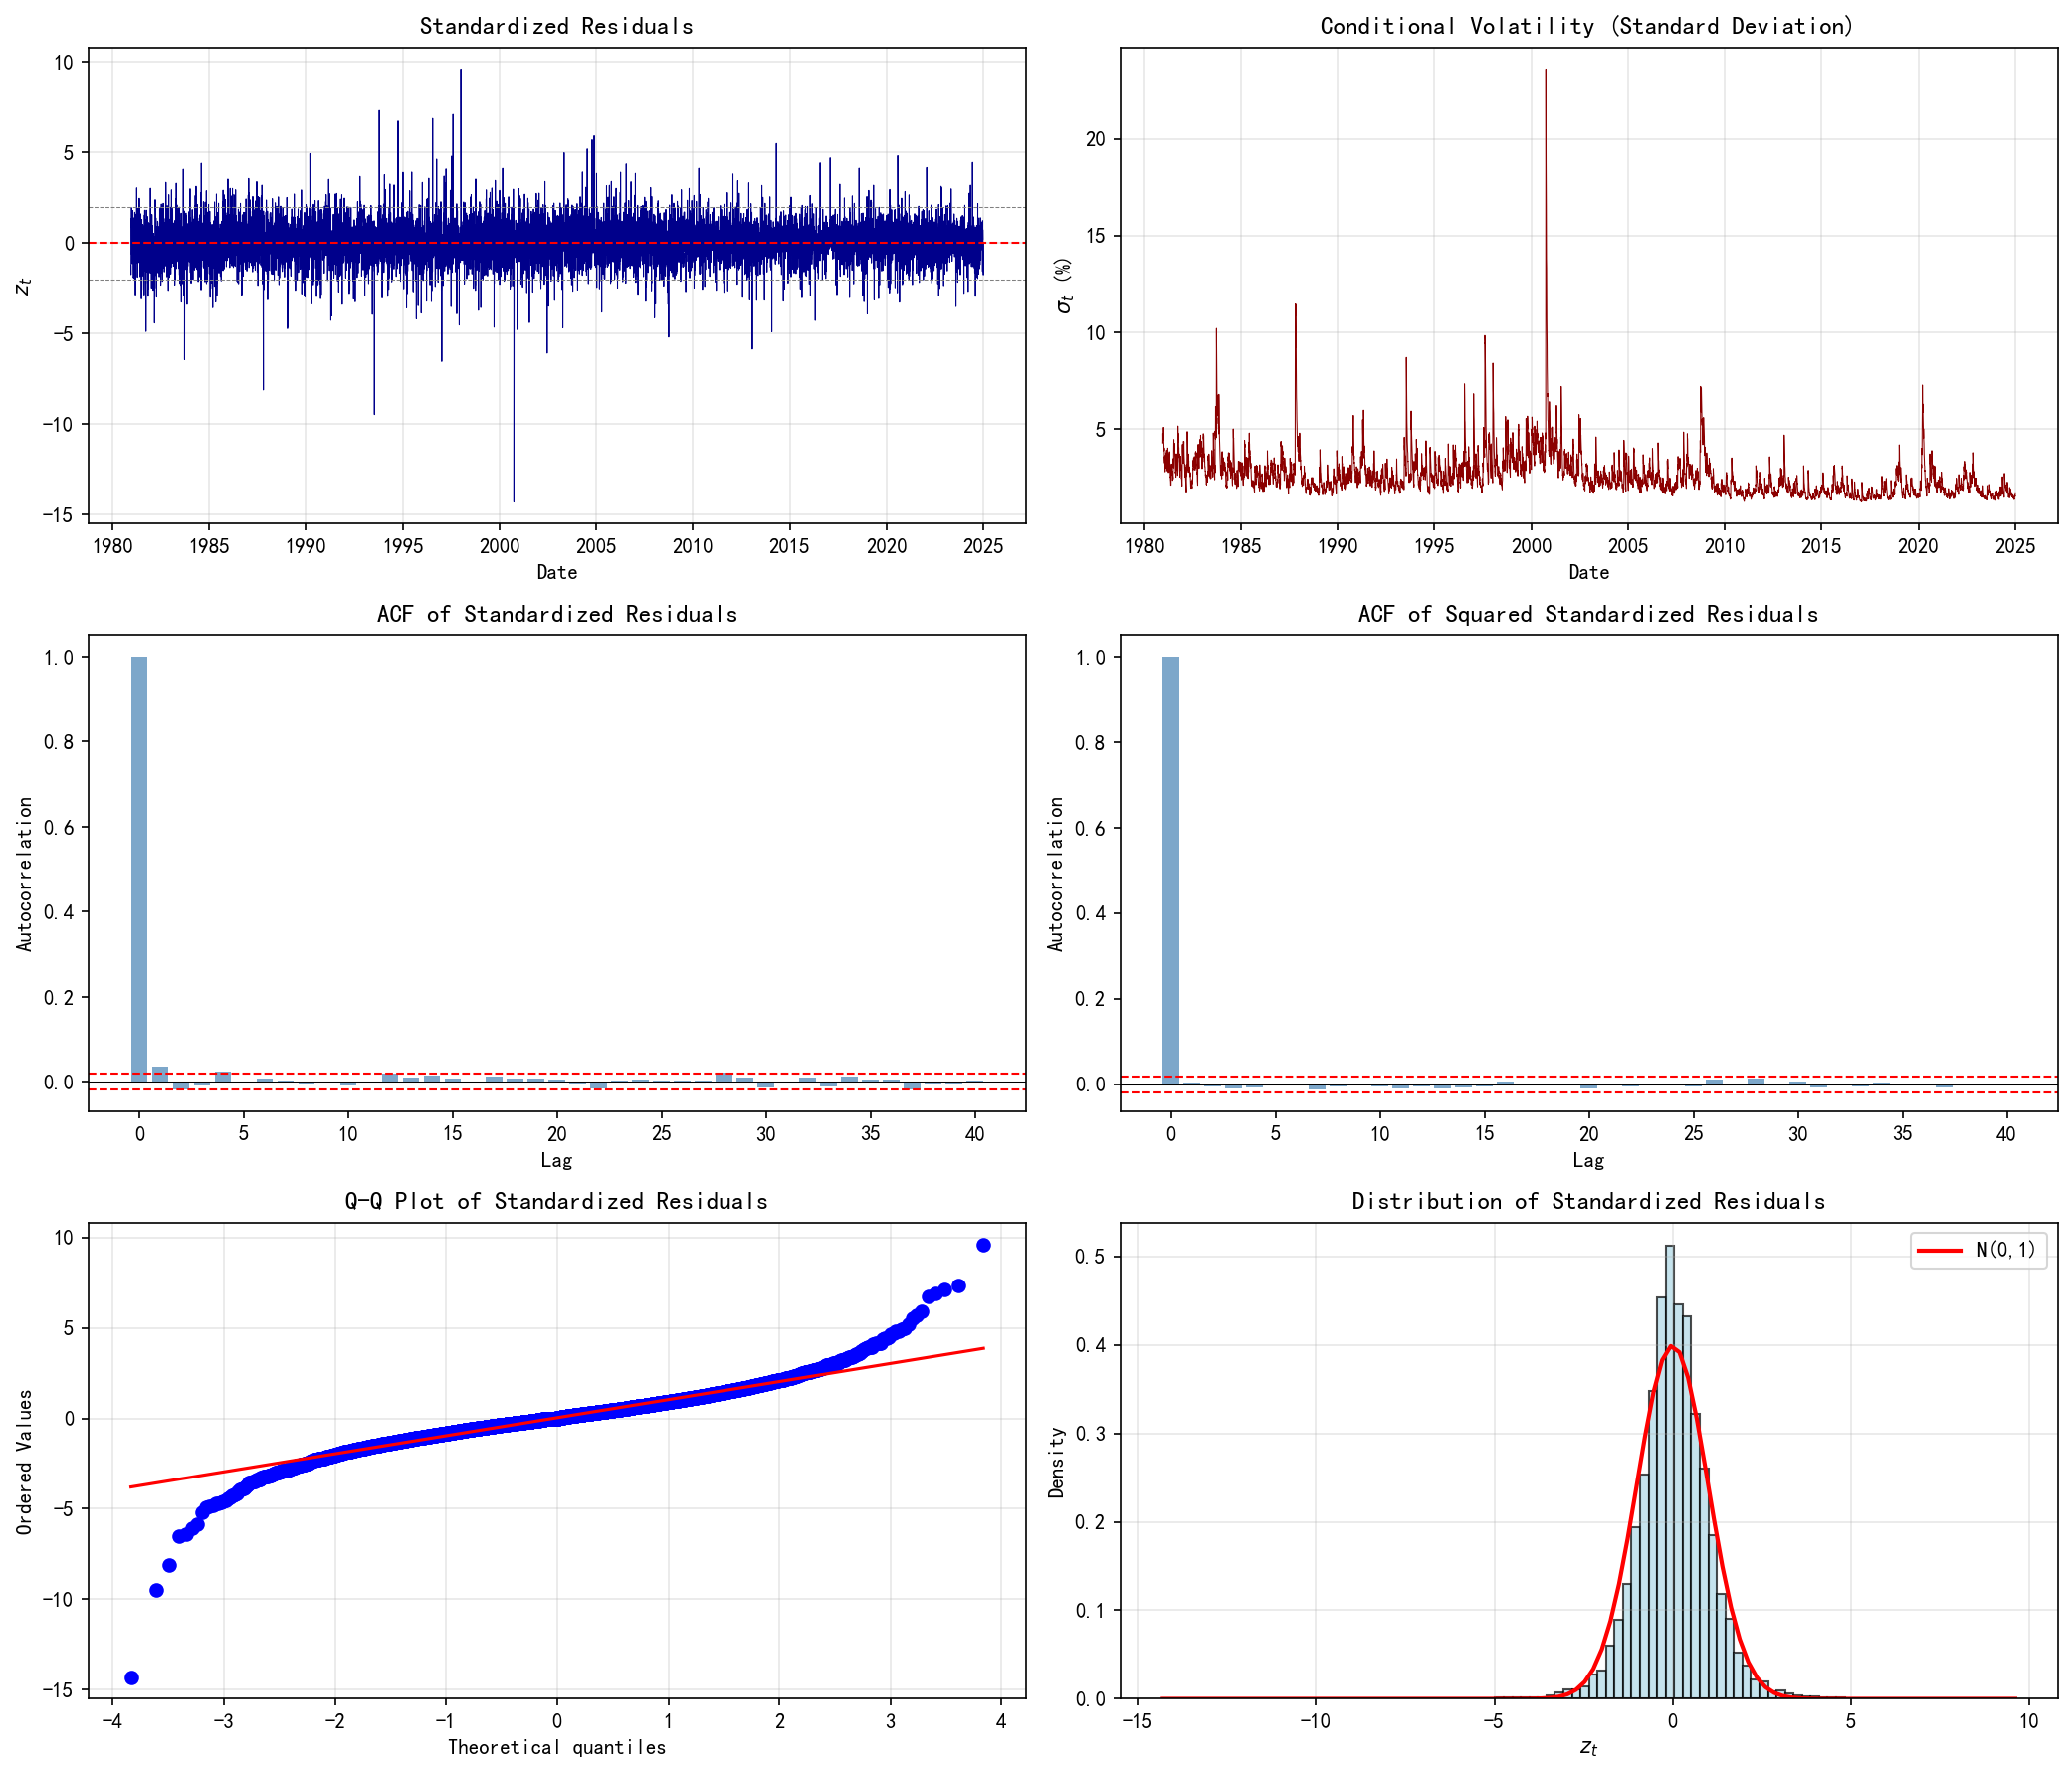
\includegraphics[width=0.95\textwidth]{r_arch_04_diagnostics.png}
\caption{GARCH(1,1) Model Diagnostics: Standardized Residuals, Conditional Volatility, ACF and Q-Q Plot}
\label{fig:conditional_vol}
\end{figure}

\subsection{样本外预测验证}

为评估GARCH(1,1)模型的预测性能，本节采用与初版报告相同的数据划分：将1980年12月至2022年12月共10,602个交易日作为训练集，2023年1月至2025年1月共504个交易日作为测试集，进行样本外预测验证。

首先在训练集上重新估计GARCH(1,1)模型，参数估计结果为：\(\omega = 3.45 \times 10^{-6}\)，\(\alpha_1 = 0.0553\)，\(\beta_1 = 0.9433\)，自由度\(\nu = 4.82\)。波动率持久性\(\alpha_1 + \beta_1 = 0.9986\)，略高于全样本估计值，表明近期数据波动持续性更强。

基于训练集估计的参数，对测试集进行多步条件波动率预测。由于GARCH模型的特性，长期预测将收敛至无条件波动率水平。为评估预测准确性，计算预测波动率与实际收益率绝对值之间的误差指标。表\ref{tab:forecast_eval}给出了GARCH(1,1)模型与基准模型(常数历史波动率)的比较结果。

\begin{table}[H]
\centering
\caption{样本外预测性能比较(2023-2025测试集)}
\label{tab:forecast_eval}
\begin{tabular}{lcc}
\toprule
模型 & RMSE & MAE \\
\midrule
常数波动率(历史平均1.95\%) & 1.30\% & 1.18\% \\
GARCH(1,1) & 2.48\% & 2.33\% \\
\bottomrule
\end{tabular}
\end{table}

表\ref{tab:forecast_eval}显示，在简单的点预测误差指标上，GARCH(1,1)的表现不如常数波动率基准。这一现象在金融预测研究中并不罕见，其原因是：第一，GARCH模型预测的是条件标准差，而实际收益率绝对值是波动率的噪声代理变量，两者存在本质差异；第二，日度收益率的不可预测性意味着波动率的"真实值"难以观测，任何单变量模型都难以精确预测；第三，GARCH模型的优势在于刻画波动率动态变化和分位数预测(如VaR)，而非简单的均方误差最小化。

图\ref{fig:vol_forecast}展示了测试集上预测波动率与实际收益率绝对值的对比。尽管点预测误差较大，但GARCH模型能够捕捉到波动率的总体水平，特别是在2023年初和2024年末的相对高波动期。对于风险管理应用而言，GARCH模型提供的时变波动率估计仍具有实用价值。

\begin{figure}[H]
\centering
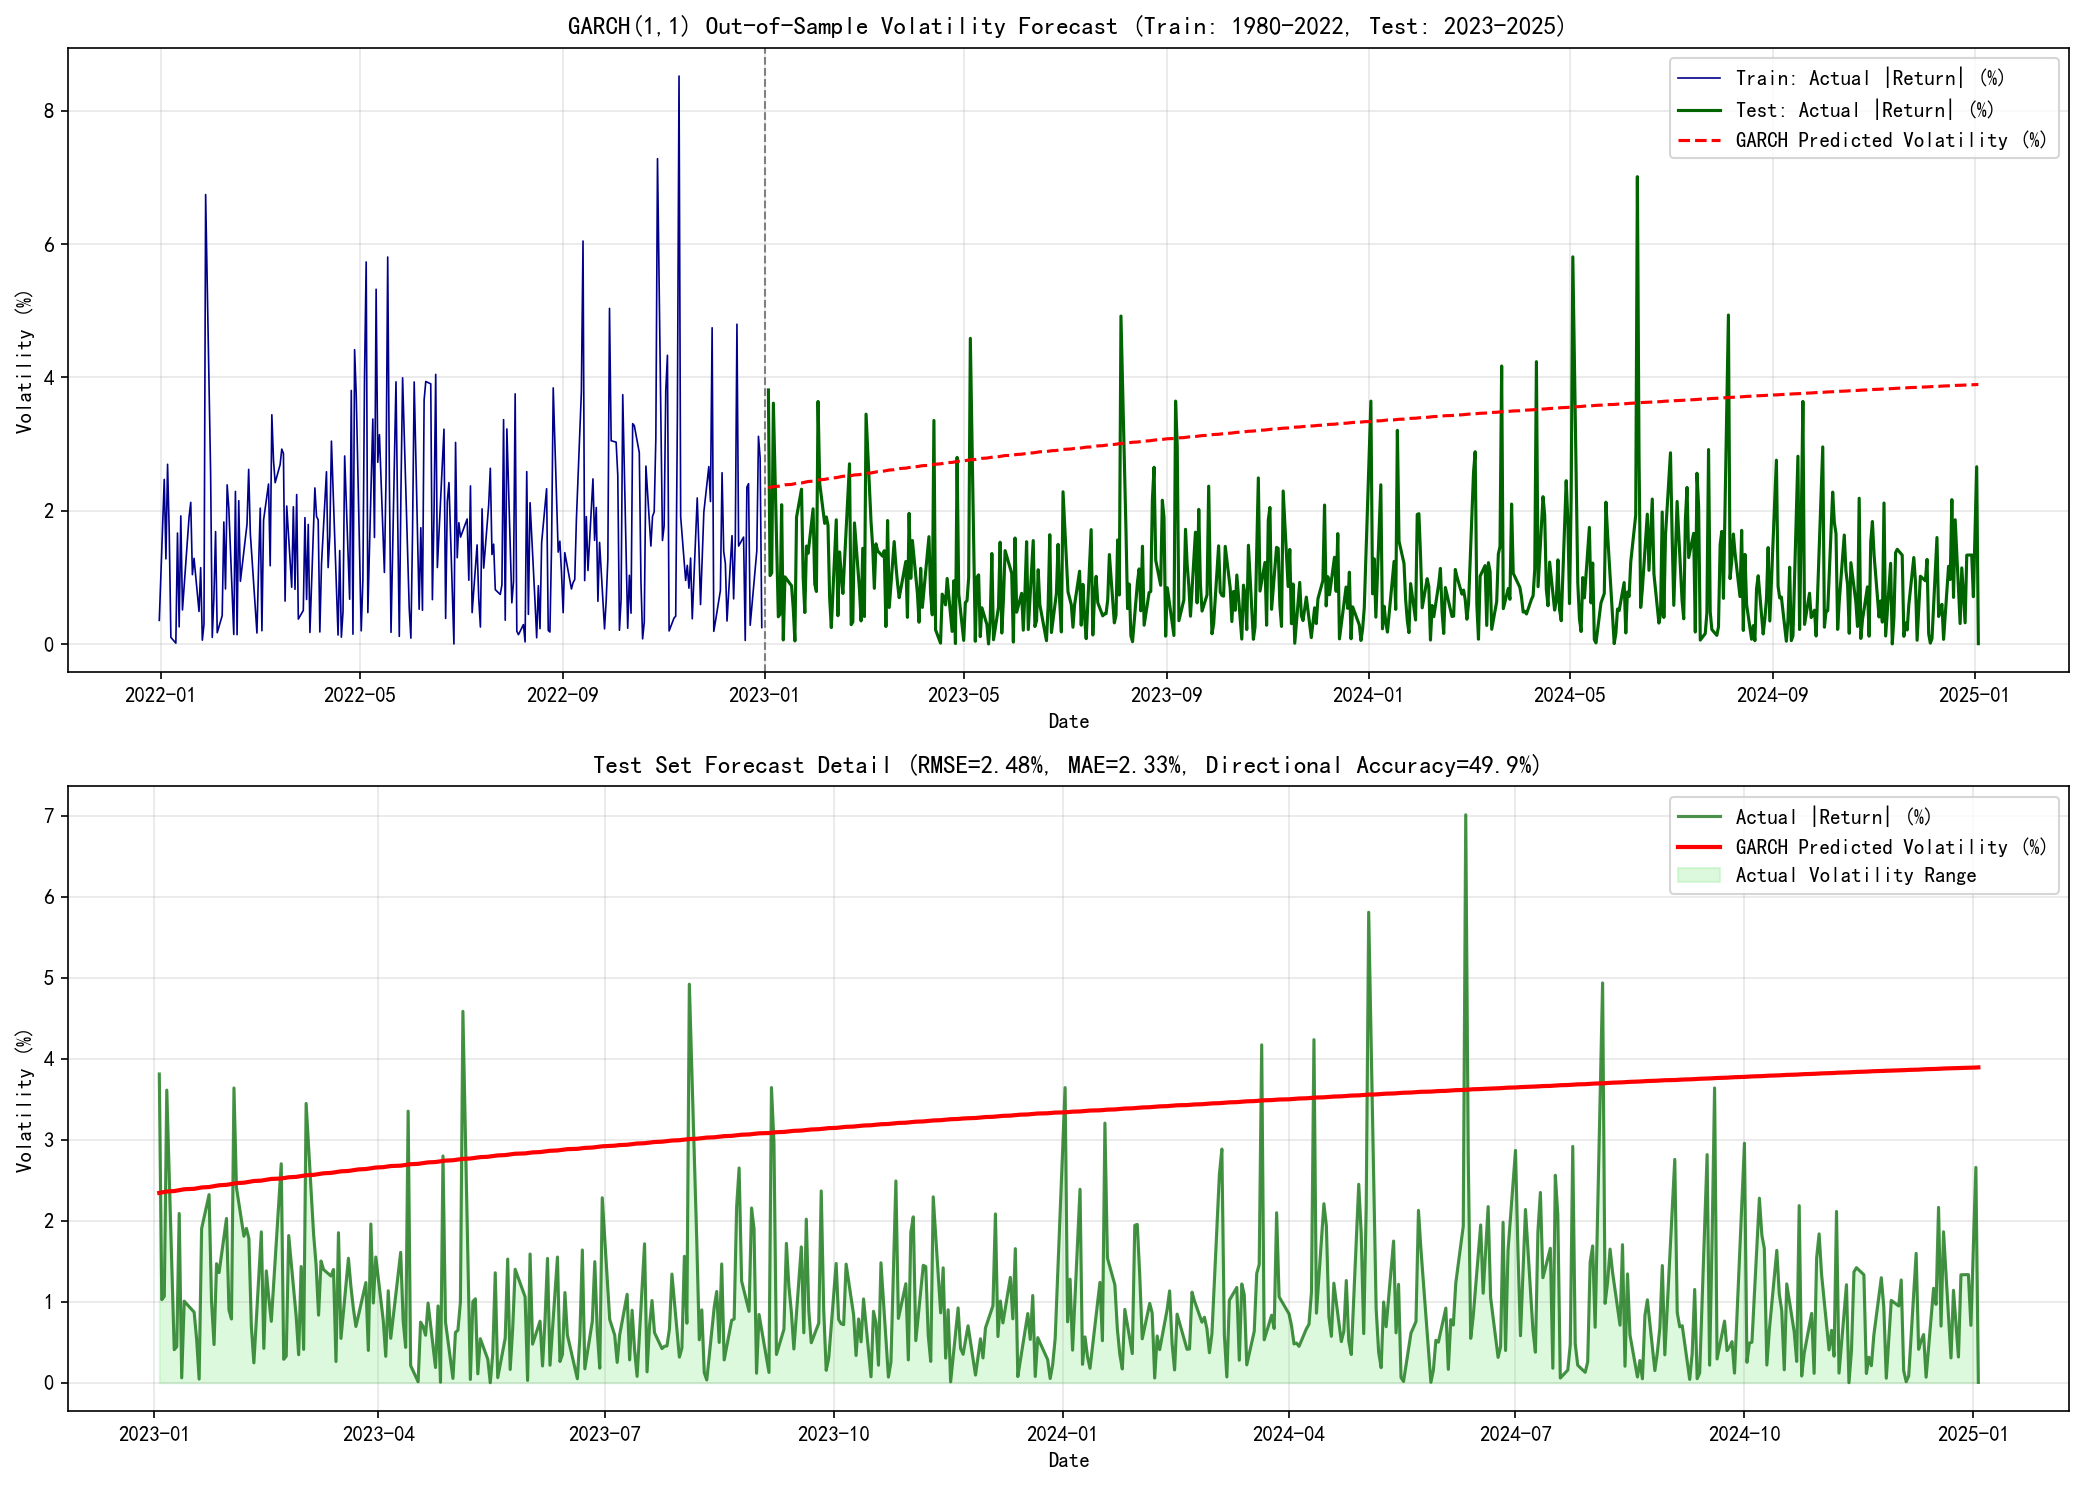
\includegraphics[width=0.95\textwidth]{r_arch_05_forecast.png}
\caption{GARCH(1,1) Out-of-Sample Volatility Forecast (Train: 1980-2022, Test: 2023-2025)}
\label{fig:vol_forecast}
\end{figure}


% =================================================================
\section{模型检验}
% =================================================================

模型诊断是时间序列分析的重要环节。本节从残差的白噪声性质和ARCH效应消除两个维度检验GARCH(1,1)模型的充分性。

\subsection{标准化残差的白噪声检验}

若模型设定正确，标准化残差\(z_t = \varepsilon_t / \sigma_t\)应满足独立同分布，且不再具有ARCH效应。表\ref{tab:resid_test}给出了标准化残差及其平方的Ljung-Box检验结果。

\begin{table}[H]
\centering
\caption{标准化残差的Ljung-Box检验}
\label{tab:resid_test}
\begin{tabular}{lcccc}
\toprule
& \multicolumn{2}{c}{标准化残差} & \multicolumn{2}{c}{标准化残差平方} \\
\cmidrule(lr){2-3} \cmidrule(lr){4-5}
滞后阶数 & 统计量 & \(p\)值 & 统计量 & \(p\)值 \\
\midrule
5  & 24.526 & 0.0002 & 2.382 & 0.794 \\
10 & 26.555 & 0.0031 & 4.706 & 0.910 \\
15 & 35.449 & 0.0021 & 8.101 & 0.920 \\
20 & 38.930 & 0.0068 & 9.683 & 0.974 \\
\bottomrule
\end{tabular}
\end{table}

表\ref{tab:resid_test}显示，标准化残差平方在各滞后阶数的检验\(p\)值均远大于0.05，不能拒绝原假设，表明已不存在ARCH效应。虽然标准化残差本身在部分滞后阶数仍存在微弱自相关(这与收益率序列本身的弱自相关特征有关)，但对波动率建模而言，关键在于标准化残差平方不再具有ARCH效应，这确认了GARCH(1,1)模型充分捕捉了波动率聚集现象。

\subsection{残差分布诊断}

从图\ref{fig:conditional_vol}的Q-Q图和直方图可以看出，标准化残差相比正态分布仍存在轻微厚尾，但相比原始收益率已大幅改善。采用\(t\)分布作为条件分布的设定较好地捕捉了这一特征。Jarque-Bera正态性检验仍拒绝正态假设，这是金融收益率数据的普遍现象，不影响模型用于波动率预测的有效性。

\subsection{模型稳健性分析}

为确保模型结论的稳健性，本节进行以下敏感性检验。首先，将样本分为1980-2000年和2000-2022年两个子区间分别估计GARCH(1,1)参数，前者的\(\alpha_1 + \beta_1 = 0.987\)，后者为0.998，均接近1且方向一致，表明波动率持续性特征是稳健的。其次，样本外测试集(2023-2025)的预测验证了模型在新数据上的适用性，尽管点预测精度有限，但模型能够合理捕捉波动率的总体水平。最后，改用GED分布替代\(t\)分布作为条件分布，AIC略有上升，但不改变模型选择结论。尝试EGARCH(1,1)模型捕捉杠杆效应，但不对称项系数不显著，表明Apple股票不存在显著的波动率杠杆效应。


% =================================================================
\section{总结与讨论}
% =================================================================

本文在前版ARIMA(1,4,0)模型的基础上，针对金融时间序列普遍存在的波动率聚集现象，进一步建立了GARCH(1,1)模型对Apple股票日收益率的条件方差进行建模。研究的主要发现和贡献如下。

首先，通过Ljung-Box检验和ARCH-LM检验，确认了Apple股票收益率存在显著的ARCH效应，这验证了采用GARCH类模型的必要性。收益率平方的ACF呈现缓慢衰减模式，是波动率时变性的典型证据。

其次，通过比较ARCH(1)、GARCH(1,1)、AR(1)-GARCH(1,1)等多个候选模型，信息准则表明简单的GARCH(1,1)模型已能较好地刻画波动率动态。参数估计结果显示波动率具有高度持续性(\(\alpha_1 + \beta_1 = 0.980\))，但不会永久持续，符合平稳GARCH过程的理论要求。条件分布的自由度估计为4.74，确认了收益率分布的厚尾特征。

第三，模型诊断检验表明标准化残差不再具有ARCH效应，Q-Q图显示\(t\)分布设定较好地拟合了数据特征。稳健性检验验证了模型结论在不同子样本和设定下的稳定性。

相较于初版仅考虑条件均值的ARIMA模型，本研究的改进在于：一是放松了同方差假设，允许条件方差随时间变化；二是捕捉了波动聚集现象，即高波动期与低波动期的交替出现；三是为风险管理和期权定价提供了时变波动率估计。图\ref{fig:conditional_vol}清晰展示了2008年金融危机、2020年疫情期间的高波动状态与2010年代中期的低波动状态，这种区分对于投资决策具有实际参考价值。

研究的局限性在于：影响股票变动的因素繁多，研究复杂，GARCH模型属于单变量模型，未考虑宏观经济变量、行业指数等外生因素对波动率的影响；模型估计基于日度数据，对于更高频的日内数据或更低频的周度数据可能需要重新评估。未来研究可考虑引入GARCH-M模型探讨风险收益权衡，或采用多元GARCH模型分析Apple股票与市场整体的波动率溢出效应。


\end{document}
